%%%DOCOCUMENT SETTINGS%%%%%%%%%%%%%%%%%%%%%%%%%%%%%%%%%%%%%%%%%%%%%%%%%%
%~ \documentclass[pdftex,12pt,a4paper,twoside]{book}
%~ \documentclass[pdftex,11pt,b5paper,twoside,draft]{book}
% \documentclass[pdftex,12pt,a4paper,twoside]{article}
\documentclass[pdftex,12pt,a4paper,oneside]{article}
\usepackage[nottoc,numbib]{tocbibind}
\usepackage{amsmath,amsfonts,amssymb,amsthm,bm,array,mathtools}
\usepackage[style=numeric,backend=biber,citestyle=chem-acs,natbib=true]{biblatex}
\usepackage[czech,british]{babel}
% \usepackage[british]{babel}
\usepackage[utf8]{inputenc}
\usepackage[T1]{fontenc}
\usepackage{fix-cm}
\usepackage{fancyhdr} %zahlavi a zapati
\usepackage[top=25.0mm, bottom=25.0mm, left=20.0mm, right=20.0mm, bindingoffset=0mm]{geometry}
%~\usepackage[top=25.4mm, bottom=25.4mm, inner=20.0mm, outer=20.0mm,bindingoffset=10mm,heightrounded,]{geometry}
\usepackage{pdflscape}
%~ \usepackage{afterpage}
\usepackage{caption,float}
\usepackage[pdftex]{graphicx}
\usepackage[protrusion=true,expansion=true]{microtype}
\usepackage{wrapfig}
\usepackage{bbold}
%~\usepackage{subfig}
%~\usepackage{subfigure}
\usepackage{xcolor}
\usepackage{lmodern} %possible to remove on linux
\usepackage{subcaption} %windows
%~\usepackage{cm-super}%windows
 %~\usepackage{subfig} %windows nefunguje
\usepackage{chemformula}
\usepackage{algorithm}
% ~\usepackage{algorithmic}
\usepackage{stmaryrd}
\usepackage[export]{adjustbox}
% \usepackage{algorithmic}
\usepackage{algpseudocode}
\usepackage{longtable}



\makeatletter\AtBeginDocument{\let\@elt\relax}\makeatother

%~\usepackage{pstricks}
%~\usepackage{auto-pst-pdf}

% CUSTOM COLORS
\definecolor{schoolColor}{HTML}{e74011} %UCT RED
%~ \definecolor{chaptergrey}{HTML}{FDB515} % chapter numbers
\definecolor{grey}{HTML}{b9b8b3} % grey
\definecolor{myPink}{HTML}{d947c8}
\definecolor{walls}{HTML}{ae7354}
\definecolor{cyl}{HTML}{b10000}
\definecolor{coat}{HTML}{0000a0}
\definecolor{violet}{HTML}{976bd9} % grey
%~\definecolor{chaptergrey}{HTML}{976bd9} % chapter numbers
\definecolor{chaptergrey}{rgb}{0.6,0.6,0.6} % chapter numbers
%~ \definecolor{myBlue1}{RGB}{0,165,211} % chapter numbers
%~ \definecolor{myBlue1}{RGB}{35,31,32} % school black
%~ \definecolor{myBlue1}{HTML}{4c4c4c} % school black
%~ \definecolor{myBlue1}{cmyk}{0.77,0.36,0,0.51}
\definecolor{myBlue1}{HTML}{2c476b}% my actual color
\newcommand\crule[3][black]{\textcolor{#1}{\rule{#2}{#3}}}
\newcommand{\missRef}{\textcolor{blue}{[REF]}}
\newcommand{\CO}{$\mathrm{CO}$}
\newcommand{\COO}{$\mathrm{CO}_{2}$}
\newcommand{\OO}{$\mathrm{O}_{2}$ }
\newcommand{\NO}{$\mathrm{NO}$}
\newcommand{\NNO}{$\mathrm{N}_{2}\mathrm{O}$}
\newcommand{\NN}{$\mathrm{N}_{2}$}
\newcommand\CFL{\mbox{\textrm{Co}}}
%~ \usepackage{sectsty}
%~ \sectionfont{\color{myBlue1}}
%~ \subsectionfont{\color{myBlue1}}
%~ \subsubsectionfont{\color{myBlue1}}
%~ \paragraphfont{\color{myBlue1}}

\usepackage[theorems,skins]{tcolorbox}
\tcbset{highlight math style={enhanced,
  colframe=myBlue1,colback=white,arc=0pt,boxrule=1pt}}

%~ \usepackage{titlesec}
%~ \titleformat{\section}
%~ {\color{red}\normalfont\Large\bfseries}
%~ {\color{red}\thesection}{1em}{}

% REFERENCING
%~ \usepackage[square,sort,comma,numbers]{natbib}
%~ \usepackage[style=numeric,backend=bibtex,natbib=true]{biblatex}
%~\usepackage[style=numeric,backend=biber,style=chem-acs,natbib=true]{biblatex}

%~\usepackage[style=numeric,backend=biber,natbib=true]{biblatex}
\bibliography{./10_bibFiles/books.bib,./10_bibFiles/references.bib,10_bibFiles/others.bib,10_bibFiles/theses.bib}
% \bibliography{./10_bibFiles/references.bib}
%~\bibliography{./10_bibFiles/books.bib,./10_bibFiles/papers.bib,10_bibFiles/others.bib}

%~ \usepackage{enumitem}
%~ \usepackage{float}
\usepackage{booktabs,multirow,bigdelim,tabularx}
%~ \usepackage{rotatingn}
\usepackage{paralist}

% ALGORITHMS
%~\usepackage{algorithm}
%~\usepackage{algcompatible}
 %~\usepackage{algpseudocode}
 %~\usepackage{algorithmic}
%~\renewcommand{\algorithmicforall}{\textbf{for each}}

% stuff due to algocompatible
%~\algnewcommand\algorithmicreturn{\textbf{return} }
%~\algnewcommand\RETURN{\State \algorithmicreturn}%
%~\newcommand{\TO}{\textbf{to }}

%~\algnewcommand{\IIf}[1]{\State\algorithmicif\ #1\ \algorithmicthen}
%~\algnewcommand{\EndIIf}{\unskip\ \algorithmicend\ \algorithmicif}

%~\makeatletter
%~\let\OldStatex\Statex
%~\renewcommand{\Statex}[1][3]{%
  %~\setlength\@tempdima{\algorithmicindent}%
  %~\OldStatex\hskip\dimexpr#1\@tempdima\relax}
%~\makeatother

%~ % PGFPLOTS AND OTHER GRAPHICS
\usepackage{nomencl}
\makenomenclature
\usepackage{pgfplotstable}
\usepackage{pgfplots}
\pgfplotsset{compat=1.9}
\usetikzlibrary{plotmarks}
\usetikzlibrary{positioning, bending}
\usetikzlibrary{patterns}
\usetikzlibrary{matrix}
\usetikzlibrary{shapes.geometric, arrows}
\usetikzlibrary{decorations.text}
\usetikzlibrary{decorations.pathreplacing}
\usepgfplotslibrary{groupplots}
\usetikzlibrary{calc}
\usetikzlibrary{decorations.pathmorphing,calc}


% \usetikzlibrary{external}
% \tikzexternalize[prefix=figures/]


\usepackage{url,etoolbox}
\preto\tabular{\shorthandoff{-}}% hack to enable cmidrule in tabs for czech/slovak
\newcolumntype{C}[1]{>{\centering\arraybackslash}p{#1}}
\usepackage{forloop}

% for plots
\definecolor{red}{RGB}{240,0,0}
\definecolor{green}{RGB}{0,220,0}
\definecolor{blue}{RGB}{100,100,220}
\definecolor{yellow}{RGB}{255,198,0}
\DeclareMathOperator{\Tr}{Tr}

\tikzstyle{startstop} = [line width = 0.75pt, ellipse, minimum width = 1cm, minimum height = 1.5cm, text centered, draw=black]
\tikzstyle{myStep} = [line width = 0.75pt, rectangle, rounded corners, minimum width = 2cm, minimum height = 0.5cm, text centered, draw=black]
\tikzstyle{counter} = [line width = 0.75pt, rectangle, dash pattern = on 4pt off 2pt, minimum width = 1cm, minimum height = 0.5cm, text centered, draw=black]
\tikzstyle{special} = [line width = 0.75pt, rectangle, rounded corners = 0.5cm, minimum width = 3.2cm, minimum height = 1.3cm, text centered, draw=black]
\tikzstyle{myText} = [line width = 0.75pt, rectangle, align = center, fill opacity = 0.0, text opacity = 1.0]
\tikzstyle{neuron} = [line width = 0.75pt, circle, minimum width = 0.8cm, minimum height = 0.8cm, text centered, draw=black]

\tikzstyle{arrow} = [line width = 0.6pt, ->, >=Stealth, shorten >= 0.05cm]
\tikzstyle{arrow2} = [line width = 0.6pt, dash pattern = on 5pt off 2pt, ->, >=Stealth, shorten >= 0.07cm, draw=yellow]
\tikzstyle{line} = [line width = 0.6pt, -]
\tikzstyle{inArrow} = [line width = 0.6pt, <-, >=Stealth, shorten <=0.07cm]
\tikzstyle{outArrow} = [line width = 0.6pt, ->, >=Stealth]

%~ %%% if you have some necessary personal definitions or packages to load, put it here
\def\myLogos{00_logos}
\def\myImg{02_images}
\def\myParts{03_parts}
\def\myGraphs{04_graphs}

\newcommand{\noteMI}[1]{\textcolor{green}{#1}} 
\newcommand{\noteTH}[1]{\textcolor{red}{#1}}


\def\bx{{\bm {x}}}
\def\bu{{\bm {u}}}
%~ \def\rd{\mathrm{d}}
%~ \def\div{\mathrm{div}}
%~ \def\grad{\mathrm{grad}}
%~ \def\bs{\bm{\mathit{S}}}
%~ \def\te{\bm{\mathsf{T}}}
%~ \def\Nabla{{\bm{\nabla}}}
%%%%%%%%%%%%%%%%%%%%%%%%%%%%%%%%%%%%%%%%%%%%%%
% for math mode
%~ \newcommand{\mbb}{\mathbb}
%~ \newcommand{\mbf}{\mathbf}
%~ \newcommand{\mathrm}{\mathrm}
%~ \newcommand{\mcal}{\mathcal}
%~ \newcommand{\mtt}{\mathtt}
%~ \newcommand{\ical}{\intercal}
% dimless numbers
\newcommand\Bond{\mbox{\textrm{Bo}}}
\newcommand\Rey{\mbox{\textrm{Re}}}
\newcommand\Co{\mbox{\textrm{Co}}}

\DeclareMathOperator*{\argmin}{argmin}
\DeclareMathOperator*{\argmax}{argmax}

%~ \makeatletter
%~ \newcommand{\leqnomode}{\tagsleft@true}
%~ \newcommand{\reqnomode}{\tagsleft@false}
%~ \makeatother{}

\makeatletter
\newcommand{\leqnomode}{\tagsleft@true\let\veqno\@@leqno}
\newcommand{\reqnomode}{\tagsleft@false\let\veqno\@@eqno}
\makeatother

% for text mode
\newcommand{\myparagraph}[1]{\paragraph{#1}\mbox{}\\\noindent}

\newtheorem{remr}{Remark}
\newtheorem{defn}{Definition}
\newtheorem{lem}{Lemma}
\newtheorem{ex}{Example}
\newtheorem{cor}{Corollary}
\newtheorem{theo}{Theorem}

\newtheorem{alg}{Algorithm}

% norm command
\newcommand{\norm}[1]{\left\lVert#1\right\rVert}


% for tables
\newcommand{\HRule}{\rule{\linewidth}{0.5mm}}

% for complex figures
\newcommand{\leftTrans}{-2.0}
\newcommand{\rightTrans}{8.70}
\newcommand{\topTrans}{6.8}
\newcommand{\botTrans}{0.8}
\newcommand{\scFact}{2.3}
% \newcommand\myApproxCG{\mathrel{\stackrel{\makebox[0pt]{\mbox{\normalfont\tiny GC}}}{$\approx$}}}
\newcommand\myApproxCG{\mathrel{\overset{\makebox[0pt]{\mbox{\normalfont\scriptsize\sffamily GQ}}}{\approx}}}
\newcommand\myApproxTE{\mathrel{\overset{\makebox[0pt]{\mbox{\normalfont\scriptsize\sffamily TE}}}{\approx}}}
\newcommand\myEqCG{\mathrel{\overset{\makebox[0pt]{\mbox{\normalfont\scriptsize\sffamily GT}}}{=}}}
\newcommand\myEqTE{\mathrel{\overset{\makebox[0pt]{\mbox{\normalfont\scriptsize\sffamily TE}}}{\approx}}}
\newcommand\myFVMar{\mathrel{\overset{\makebox[0pt]{\mbox{\normalfont\scriptsize\sffamily FVM}}}{\rightarrow}}}

%% set up the colors %%%%%%%%%%%%%%%%%%%%%%%%%%%%%%%%%%%%%%%%%%%%%%%%%%%

% section and lower
%~ \makeatletter
%~ \renewcommand\thesection       {{\color{chaptergrey}\arabic{section}}}
%~ \renewcommand\thesubsection    {\thesection{\color{chaptergrey}.\arabic{subsection}}}
%~ \renewcommand\thesubsubsection {\thesubsection {\color{chaptergrey}.\arabic{subsubsection}}}
%~ \renewcommand\theparagraph     {\thesubsubsection{\color{chaptergrey}.\arabic{paragraph}}}
%~ \renewcommand\thesubparagraph  {\theparagraph{\color{chaptergrey}.\arabic{subparagraph}}}
%~ 
%~ 
%~ \makeatother

% pagestyle empty settings
\addtocontents{toc}{\protect\thispagestyle{empty}}

% paragraph settings
\setlength{\parskip}{\baselineskip}%
\setlength{\parindent}{0pt}%

    

\usepackage{nameref}
\usepackage{hyperref}%with borders around refs
\hypersetup{
    bookmarks=true,         % show bookmarks bar?
    unicode=true,          % non-Latin characters in Acrobat’s bookmarks
    pdftoolbar=true,        % show Acrobat’s toolbar?
    pdfmenubar=true,        % show Acrobat’s menu?
    pdffitwindow=true,     % window fit to page when opened
    pdfstartview={FitH},    % fits the width of the page to the window
    pdftitle={nameOfTheWorkHere},    % title
    pdfauthor={author},     % author
    pdfsubject={Masters thesis},   % subject of the document
    pdfcreator={},   % creator of the document
    pdfproducer={}, % producer of the document
    pdfkeywords={}, % list of keywords
    pdfnewwindow=true,      % links in new window
    colorlinks=true,       % false: boxed links; true: colored links
    linkcolor=black,          % color of internal links
    citecolor=black,        % color of links to bibliography
    filecolor=black,      % color of file links
    urlcolor=black           % color of external links
} 
%%%%%%%%%%%%%%%%%%%%%%%%%%%%%%%%%%%%%%%%%%%%%%
                                                      %packages and general
% redefine \mathrm to be a \protected macro rather than a `robust' command
\protected\edef\mathrm{%
  \unexpanded\expandafter\expandafter\expandafter{%
    \csname mathrm \endcsname
  }%
}

\newcommand{\numOfFiles}{11}
\newcommand{\figHeight}{8cm}
\newcommand{\figWidth}{8cm}

\newcounter{cnt}
\newcommand\textlist{}
\newcommand\settext[2]{%
  \csdef{text#1}{#2}}
\newcommand\addtext[1]{%
  \stepcounter{cnt}%
  \csdef{text\thecnt}{#1}}
\newcommand\gettext[1]{%
  \csuse{text#1}}
  
\newcounter{savePage}
  
%% Adds a possibility of setting the cycle position %%%%%%%%%%%%%%%%%%%%
\makeatletter
\def\pgfplots@getautoplotspec into#1{%
    \begingroup
    \let#1=\pgfutil@empty
    \pgfkeysgetvalue{/pgfplots/cycle multi list/@dim}\pgfplots@cycle@dim
    %
    \let\pgfplots@listindex=\pgfplots@numplots
    %%% Start new code
    \pgfkeysgetvalue{/pgfplots/cycle list set}\pgfplots@listindex@set
    \ifx\pgfplots@listindex@set\pgfutil@empty
    \else 
        \c@pgf@counta=\pgfplots@listindex
        \c@pgf@countb=\pgfplots@listindex@set
        \advance\c@pgf@countb by -\c@pgf@counta
        \globaldefs=1\relax
        \edef\setshift{%
            \noexpand\pgfkeys{
                /pgfplots/cycle list shift=\the\c@pgf@countb,
                /pgfplots/cycle list set=
            }
        }%
        \setshift%
    \fi
    %%% End new code    
    \pgfkeysgetvalue{/pgfplots/cycle list shift}\pgfplots@listindex@shift
    \ifx\pgfplots@listindex@shift\pgfutil@empty
    \else
        \c@pgf@counta=\pgfplots@listindex\relax
        \advance\c@pgf@counta by\pgfplots@listindex@shift\relax
        \ifnum\c@pgf@counta<0
            \c@pgf@counta=-\c@pgf@counta
        \fi
        \edef\pgfplots@listindex{\the\c@pgf@counta}%
    \fi
    \ifnum\pgfplots@cycle@dim>0
        % use the 'cycle multi list' feature.
        %
        % it employs a scalar -> multiindex map like
        % void fromScalar( size_t d, size_t scalar, size_t* Iout, const size_t* N )
        % {
        %   size_t ret=scalar;
        %   for( int i = d-1; i>=0; --i ) {
        %       Iout[i] = ret % N[i];
        %       ret /= N[i];
        %   }
        % }
        % to get the different indices into the cycle lists.
        %-------------------------------------------------- 
        \c@pgf@counta=\pgfplots@cycle@dim\relax
        \c@pgf@countb=\pgfplots@listindex\relax
        \advance\c@pgf@counta by-1
        \pgfplotsloop{%
            \ifnum\c@pgf@counta<0
                \pgfplotsloopcontinuefalse
            \else
                \pgfplotsloopcontinuetrue
            \fi
        }{%
            \pgfkeysgetvalue{/pgfplots/cycle multi list/@N\the\c@pgf@counta}\pgfplots@cycle@N
            % compute list index:
            \pgfplotsmathmodint{\c@pgf@countb}{\pgfplots@cycle@N}%
            \divide\c@pgf@countb by \pgfplots@cycle@N\relax
            %
            \expandafter\pgfplots@getautoplotspec@
                \csname pgfp@cyclist@/pgfplots/cycle multi list/@list\the\c@pgf@counta @\endcsname
                {\pgfplots@cycle@N}%
                {\pgfmathresult}%
            \t@pgfplots@toka=\expandafter{#1,}%
            \t@pgfplots@tokb=\expandafter{\pgfplotsretval}%
            \edef#1{\the\t@pgfplots@toka\the\t@pgfplots@tokb}%
            \advance\c@pgf@counta by-1
        }%
    \else
        % normal cycle list:
        \pgfplotslistsize\autoplotspeclist\to\c@pgf@countd
        \pgfplots@getautoplotspec@{\autoplotspeclist}{\c@pgf@countd}{\pgfplots@listindex}%
        \let#1=\pgfplotsretval
    \fi
    \pgfmath@smuggleone#1%
    \endgroup
}

\pgfplotsset{
    cycle list set/.initial=
}
\makeatother
%%%%%%%%%%%%%%%%%%%%%%%%%%%%%%%%%%%%%%%%%%%%%%%%%%%%%%%%%%%%%%%%%%%%%%%%

\pgfplotsset{
/pgfplots/bar cycle list/.style={/pgfplots/cycle list={%
cyan!60!black,fill=cyan!80!black,mark=none*\\%
lime!80!black,fill=lime,mark=none*\\%
red,densely dashed,fill=red!80!black,mark=none*\\%
yellow!60!black,densely dashed,solid,fill=yellow!80!black,mark=none*\\%
black,solid,fill=gray,mark=none*\\%
red,densely dashed,fill=red!80!black,mark=mark=none*\\%
}
},
}
\pgfplotsset{soldot/.style={color=black,only marks,mark=*},
             holdot/.style={color=black,fill=white,only marks,mark=*},
             compat=1.12}

% Style to select only points from #1 to #2 (inclusive)
\pgfplotsset{select coords between index/.style 2 args={
    x filter/.code={
        \ifnum\coordindex<#1\def\pgfmathresult{}\fi
        \ifnum\coordindex>#2\def\pgfmathresult{}\fi
    }
}}

\pgfdeclarelayer{bg}    % declare background layer
\pgfsetlayers{bg,main}  % set the order of the layers (main is the standard layer

\tikzset{>=latex}

% \newbox{\LegDas}
% \savebox{\LegDas}{
%     (\begin{tikzpicture}
%     \draw[black,thick,dashdotted](0,0.09) -- (0.5,0.09);
%     \phantom{\draw[white](0,0) -- (0.09,0);}
%     \end{tikzpicture})}

% \newbox{\LegDash}
% \savebox{\LegDash}{
%     (\begin{tikzpicture}
%     \draw[black,thick,dashed](0,0.09) -- (0.55,0.09);
%     \phantom{\draw[white](0,0) -- (0.09,0);}
%     \end{tikzpicture})}
                                               %pgfplot library settings
%%%DOCUMENT ITSELF%%%%%%%%%%%%%%%%%%%%%%%%%%%%%%%%%%%%%%%%%%%%%%%%%%%%%%
\thispagestyle{empty}
\pagenumbering{gobble}

\begin{document}

%%%TITLEPAGE%%%%%%%%%%%%%%%%%%%%%%%%%%%%%%%%%%%%%%%%%%%%%%%%%%%%%%%%%%%%
% \selectlanguage{british}

\begin{titlepage}

\hspace{5.5cm}

% Head

\includegraphics[height=1.4cm]{\myLogos/logoUCT_basic_CB.png} \\[0.3cm]

%~ \textbf{\normalsize{UNIVERSITY OF CHEMISTRY AND TECHNOLOGY, PRAGUE}\\[0.5cm]
\color{black!60}\Large\textsf{Institute of Thermomechanics, Czech Academy of Sciences}\\[0.4cm]
\color{black}
{\fontsize{16}{60}\selectfont \textbf{{\textsf{Department of Waves in Solids}}}\\[0.6cm]}


% Title
{\fontsize{35}{60}\selectfont {\textsf{Air flow in the urban area of\\[0.15cm]Hsinchu city}\\[0.4cm]}}

{{\Large \textsf{REPORT FROM THE STUDENT INTERNSHIP}}\\[0.4cm]}

\vfill

% Author and supervisor
\begin{tabular}{p{0.2\textwidth}|p{0.8\textwidth}}
\textsf{\small\color{chaptergrey}AUTHOR}         &   \textbf{\Large\textsf{Ing. Tomáš Hlavatý}}\\[0.1cm]
% \textsf{\small\color{chaptergrey}SUPERVISOR}     &   \textbf{\Large\textsf{Ing. Martin Isoz, Ph.D.}}\\[0.1cm]
% \textsf{\small\color{chaptergrey}STUDY FIELD}  &   \textbf{\Large\textsf{Chemical Engineering and Bioengineering}}\\[0.1cm]
\textsf{\small\color{chaptergrey}PROGRAMME}    &   \textbf{\Large\textsf{NARLabs student internship programme}}\\[0.1cm]
\textsf{\small\color{chaptergrey}YEAR}           &   \textbf{\Large\textsf{2023}}
\end{tabular}

\end{titlepage}

%%%ABSTRACT%%%%%%%%%%%%%%%%%%%%%%%%%%%%%%%%%%%%%%%%%%%%%%%%%%%%%%%%%%%%%
\cleardoublepage
\section*{Summary}
\noteTH{Abstract of the report will be there}

%%%NICE IMAGE AND DEDICATION%%%%%%%%%%%%%%%%%%%%%%%%%%%%%%%%%%%%%%%%%%%%
\cleardoublepage
\phantom{a}
\vfill

\section*{Acknowledgements}
\noteTH{Acknowledgements for supervisors and the NARLabs.}

%%%TABLE-OF-CONTENTS%%%%%%%%%%%%%%%%%%%%%%%%%%%%%%%%%%%%%%%%%%%%%%%%%%%%
\cleardoublepage
\tableofcontents

%%%INCLUDE TEXT PARTS%%%%%%%%%%%%%%%%%%%%%%%%%%%%%%%%%%%%%%%%%%%%%%%%%%%
\cleardoublepage
\pagenumbering{arabic}
\section{Introduction}
\label{sec:intro}

\noteTH{Introduction here}
\cleardoublepage
\section{Theoretical part}
\label{sec:theor}

\noteTH{Theoretical part here}
\cleardoublepage

\section{Used computational evironment setup}
\label{sec:env}

NCHC servers use singularity container~\cite{singularity}.

\subsection{Preparation of the singularity container}
\label{subsec:prepCont}

Assuming you have super-user permission and singularity installed, a preparation of the singularity container image from docker ubuntu:latest release and with openfoam.org/v10 and other useful applications installed inside can be done as follows:
\begin{itemize}
    \item New container (\texttt{./ubuntu}) is created from ubuntu docker repository, \texttt{----sandbox} flag allows to write into it later:\\[0.2cm] 
    \texttt{sudo singularity build --sandbox ./ubuntu docker://ubuntu:latest}
    \item Shell inside container is opened with \texttt{----writable} flag to install necessary stuff into container:\\[0.2cm] 
    \texttt{sudo singularity shell --writable ./ubuntu}
    \item Installation of the basic applications and openfoam.org/v10 into container:\\[0.2cm] 
    \texttt{apt update}\\
    \texttt{apt install python3 python3-pip wget vim software-properties-common \\ \indent\quad\quad python3-tk}\\
    \texttt{pip3 install matplotlib}\\
    \texttt{sh -c "wget -O - https://dl.openfoam.org/gpg.key >} \\ \indent\quad\quad\texttt{/etc/apt/trusted.gpg.d/openfoam.asc"}\\
    \texttt{add-apt-repository http://dl.openfoam.org/ubuntu}\\
    \texttt{apt update}\\
    \texttt{apt install openfoam10}
    \item If you want to compile custom openfoam solver, source openfoam in container:\\[0.2cm] 
    \texttt{. /opt/openfoam10/etc/bashrc}
    \item and compile it using \texttt{wmake} in prepared solver directory (in our case in\\ \texttt{./01\_codes/OF\_cases/03\_customSolvers/pollutionFoam}).
    \item When everything is installed, the \texttt{.sif} container file can be build using:\\[0.2cm] 
    \texttt{sudo singularity build ubuntu.sif ./ubuntu/}
\end{itemize}

Following the above listed guideline, singularity container image \texttt{ubuntu.sif} is created. This can be deported to NCHC servers and used. 


\section{Model description}
\label{sec:modDesc}

\noteTH{Models description here.}
\cleardoublepage
\section{Example tutorial case results}
\label{sec:exp}

In the present section the results of the chosen example tutorial case are presented. The simulation of the flow, and the air pollution spreading are performed in the segregated manner. 

Firstly, we focus onto the flow results, i.e.\ the solution of~(\ref{eq:RANS1},~\ref{eq:RANS2}). The simulation run in parallel utilizing 12 cores of the Taiwania-3 server~\cite{tw3} for approximately 4 hours.  The resulting stream-wise velocity component contours ($u_x$) on the $y$-normal slice, and the pressure contours ($p$) on the ground computational domain boundary ($\partial\Omega_{\mathrm{g}}$) are presented in Figure~\ref{fig:ux_p}a. 

\begin{figure}[htpb]
    \begin{tikzpicture}
        \node (up) {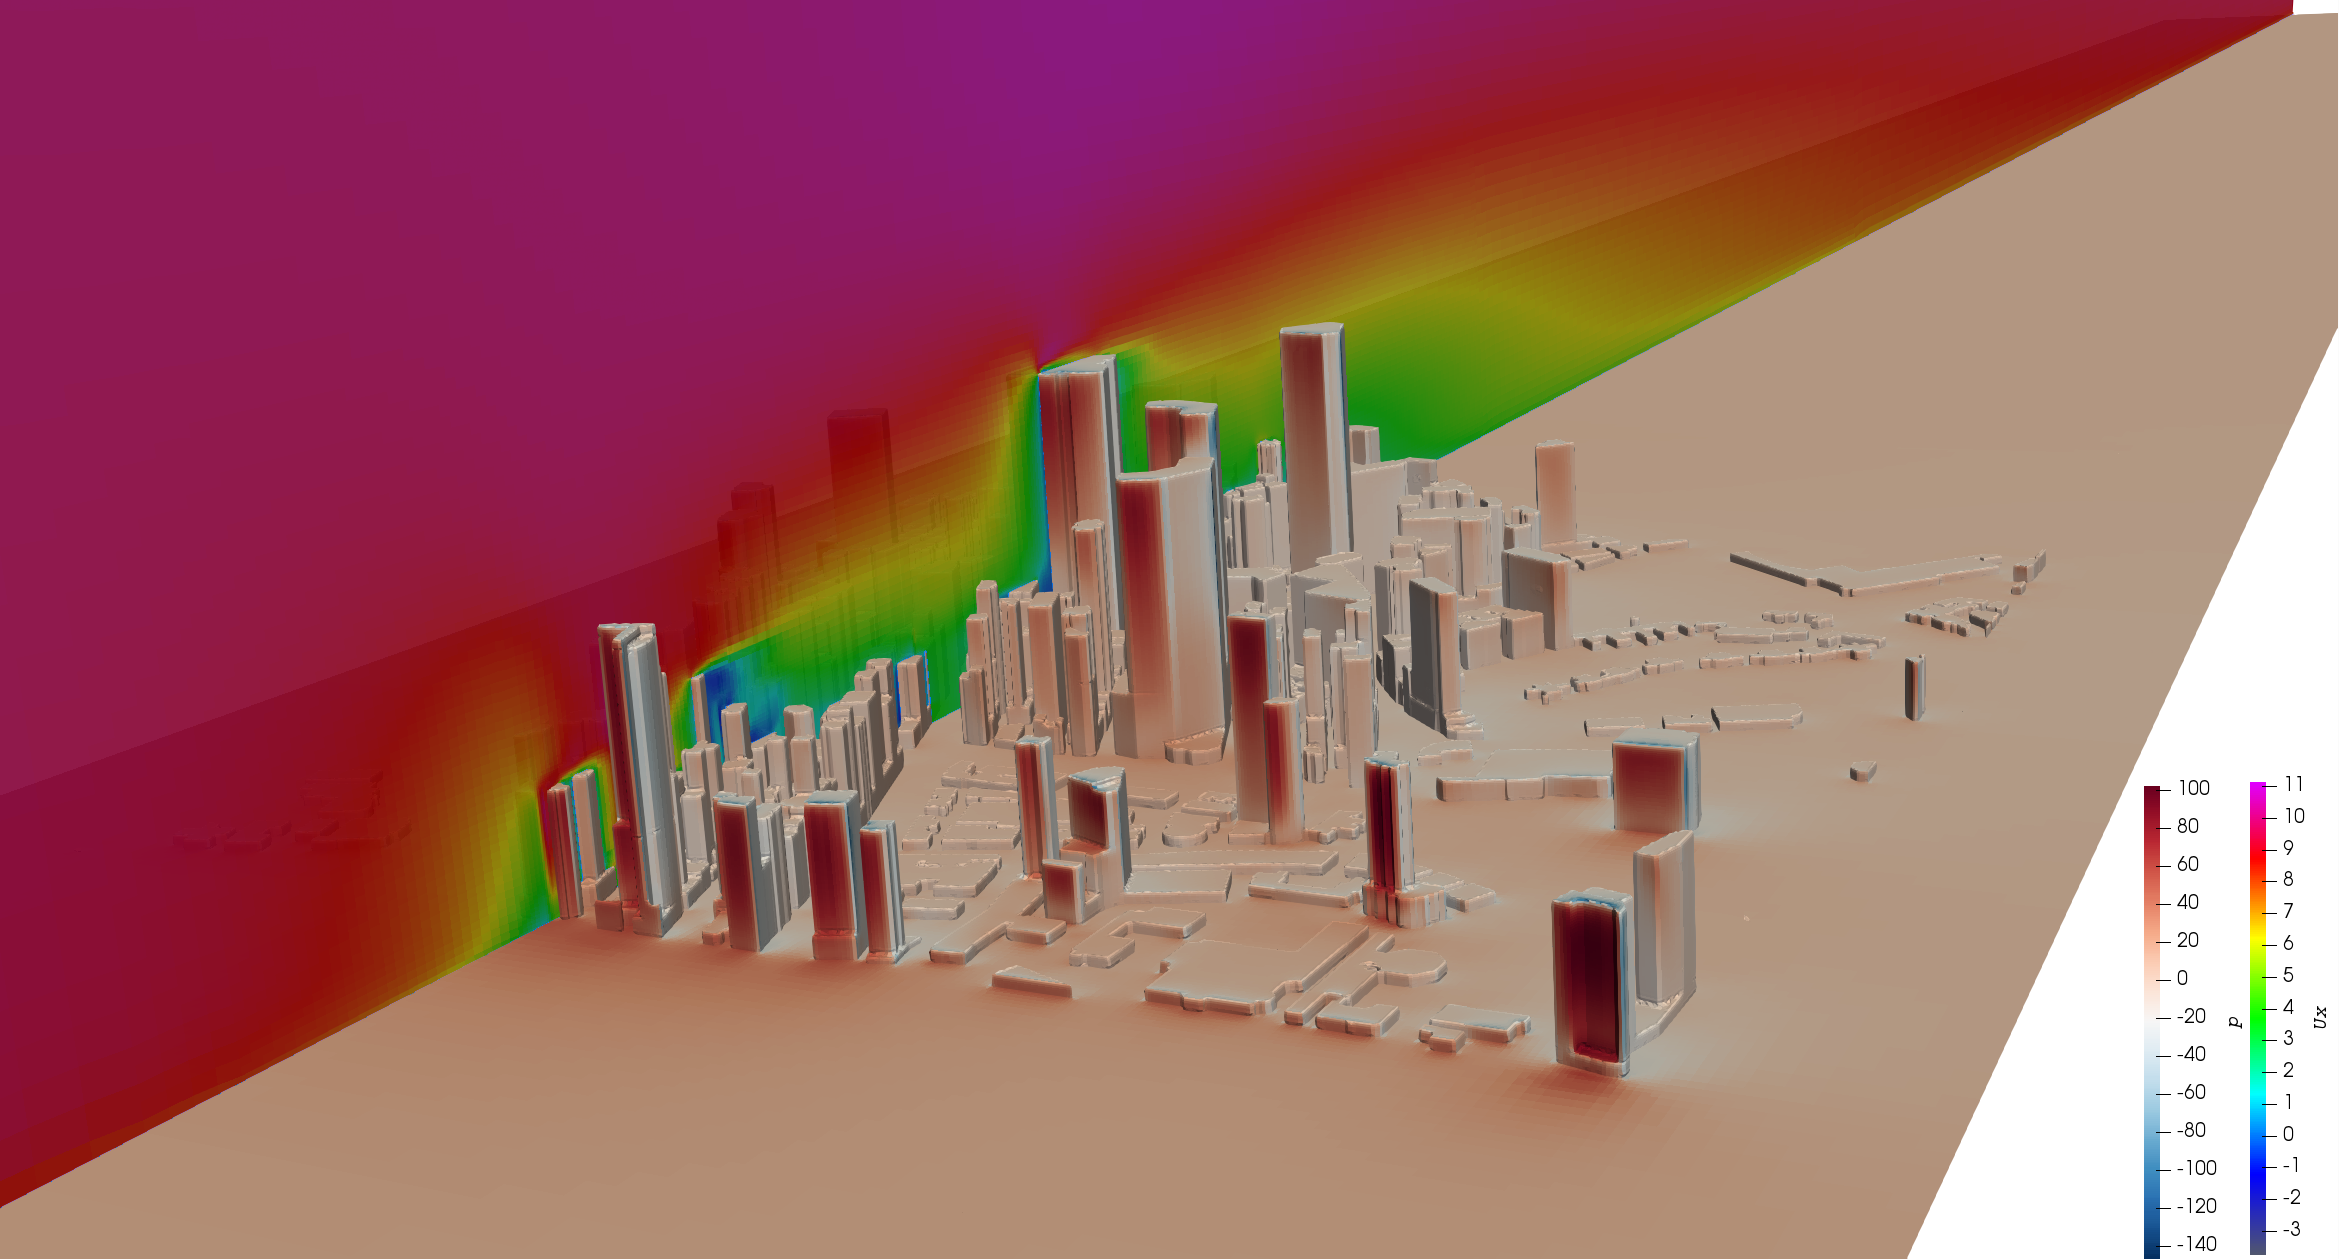
\includegraphics[width=0.95\textwidth]{01_images/res/pUxFront2.png}};
        \node at (up.north west) [anchor=north west, color=white, shift={(0.2cm,0-0.2cm)}] {a)}; 
        \node (down) at (up.south) [anchor=north] {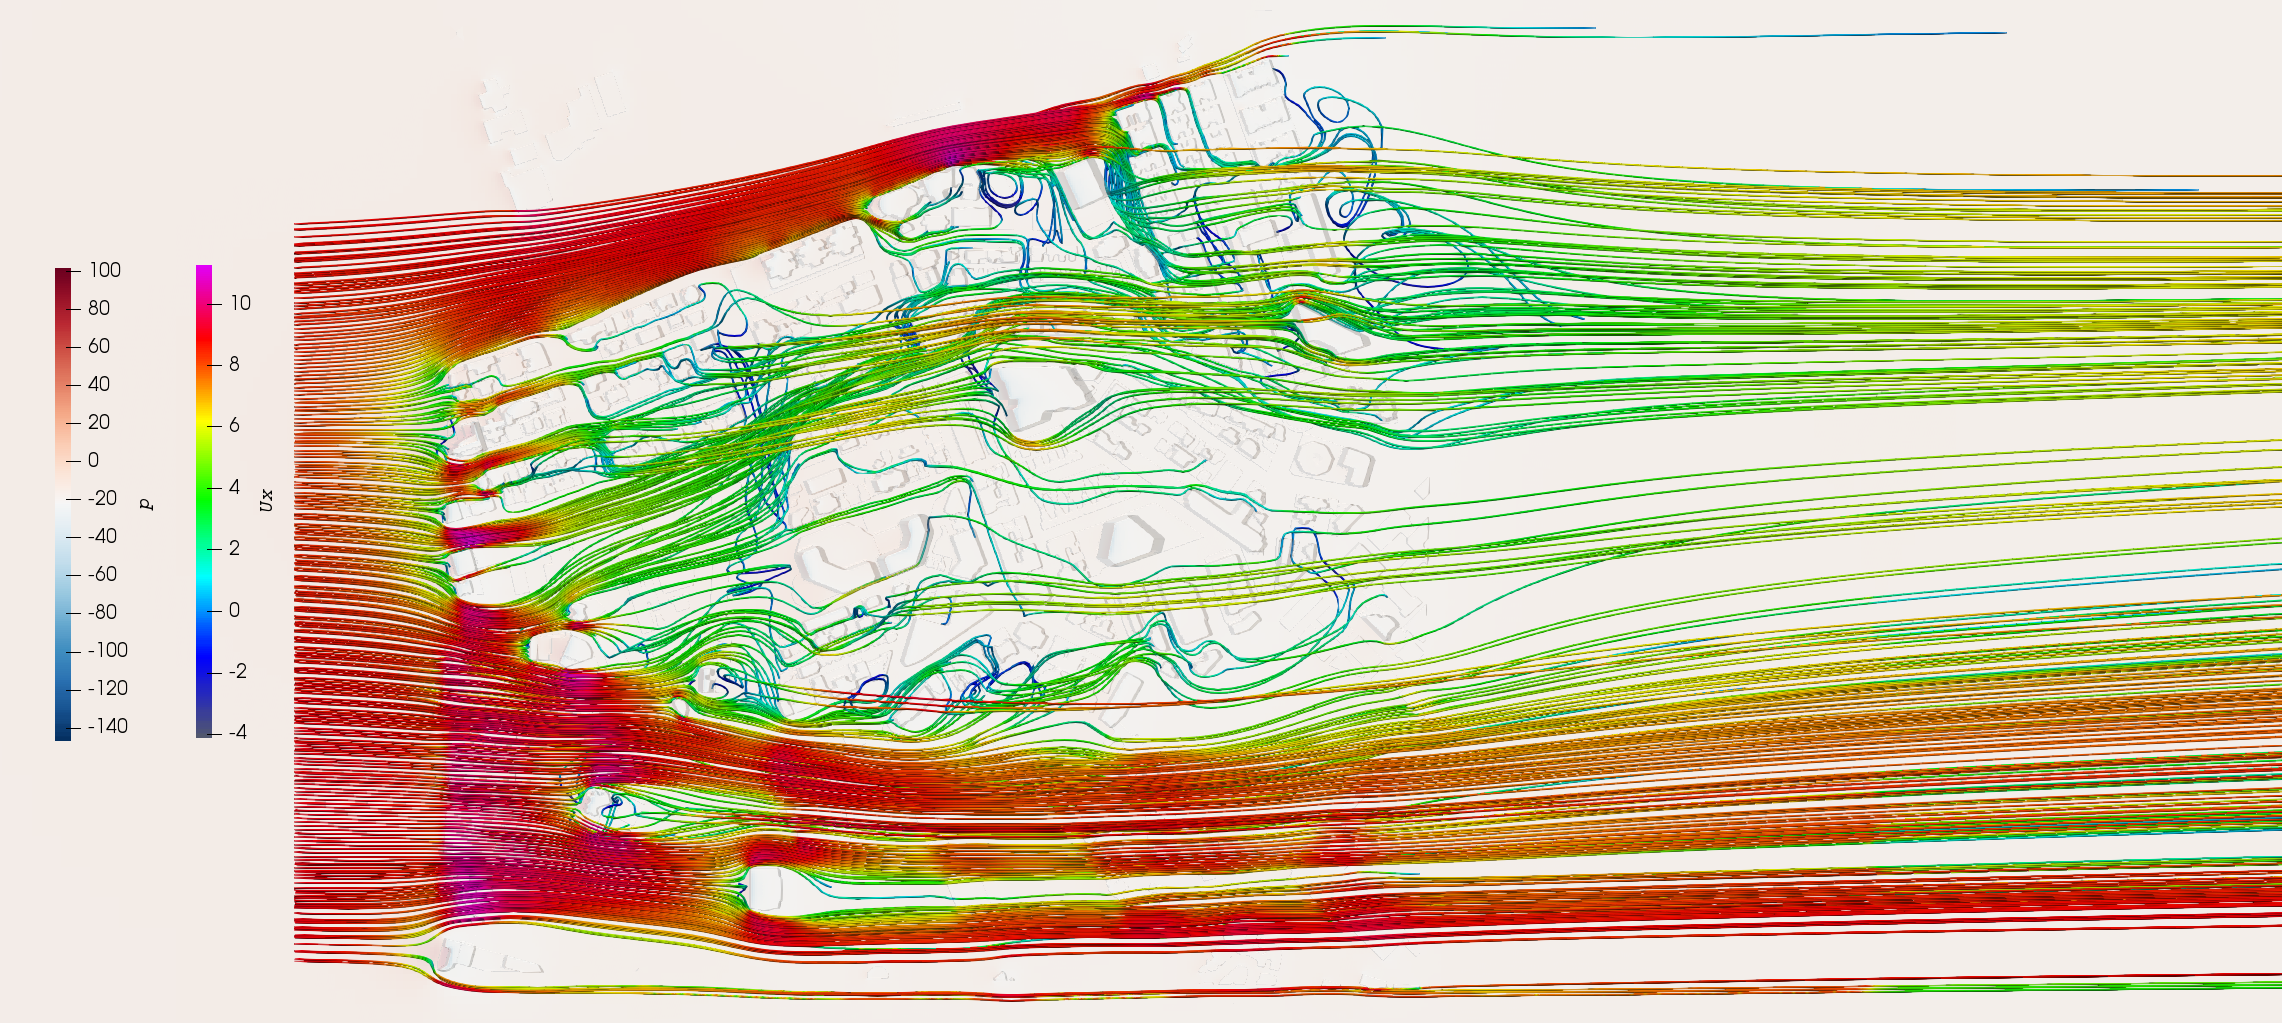
\includegraphics[width=0.95\textwidth]{01_images/res/streamUp2.png}};
        \node at (down.north west) [anchor=north west,shift={(0.2cm,0-0.2cm)}] {b)};
    \end{tikzpicture}
    
    \caption{a) Stream-vise velocity component ($u_x$), and pressure ($p$) contours on $y$-normal slice, and the ground boundary, respectively, b) main flow pathways visualized using flow streamlines colored by streamwise velocity component.}
    \label{fig:ux_p}
\end{figure}

\begin{figure}[htpb]
    \begin{tikzpicture}
        \node (left) {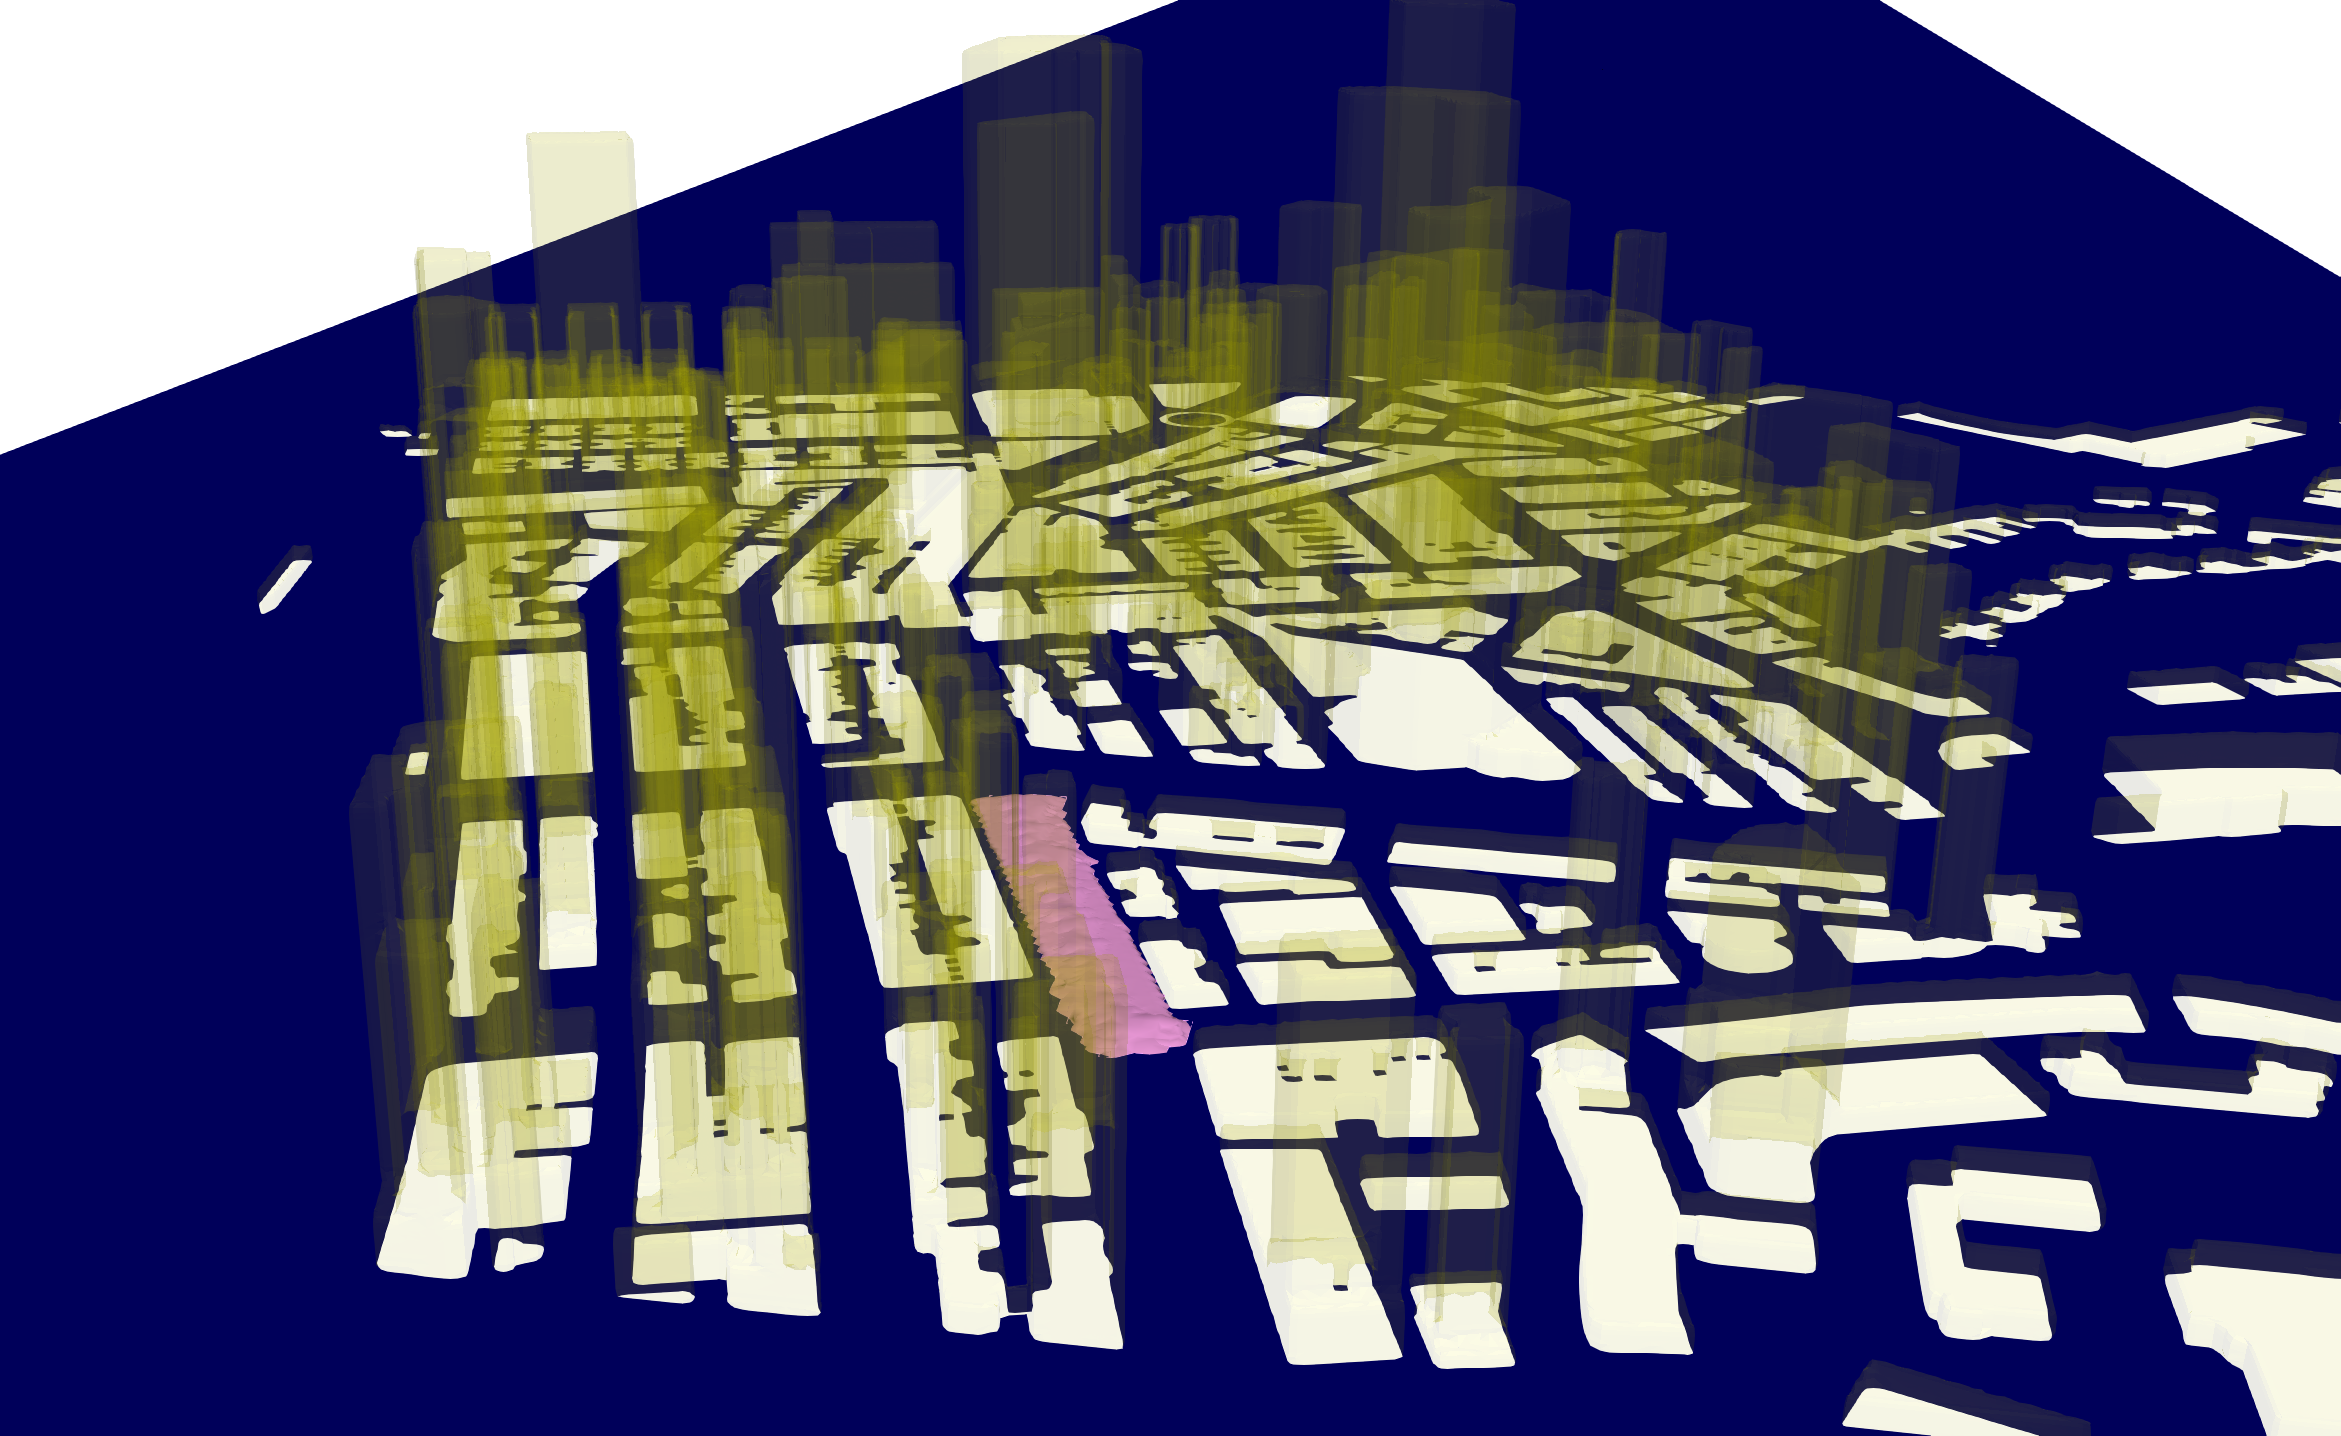
\includegraphics[width = 0.5\textwidth, trim={0 50px 0 200px},clip]{01_images/anim/animV1.0002.png}};
        \node at (left.west) [anchor=north, xshift = 0.2cm, rotate=90, color=white] {$t$ = 1\,s};
        % \node (right) at (left.east) [anchor=west] {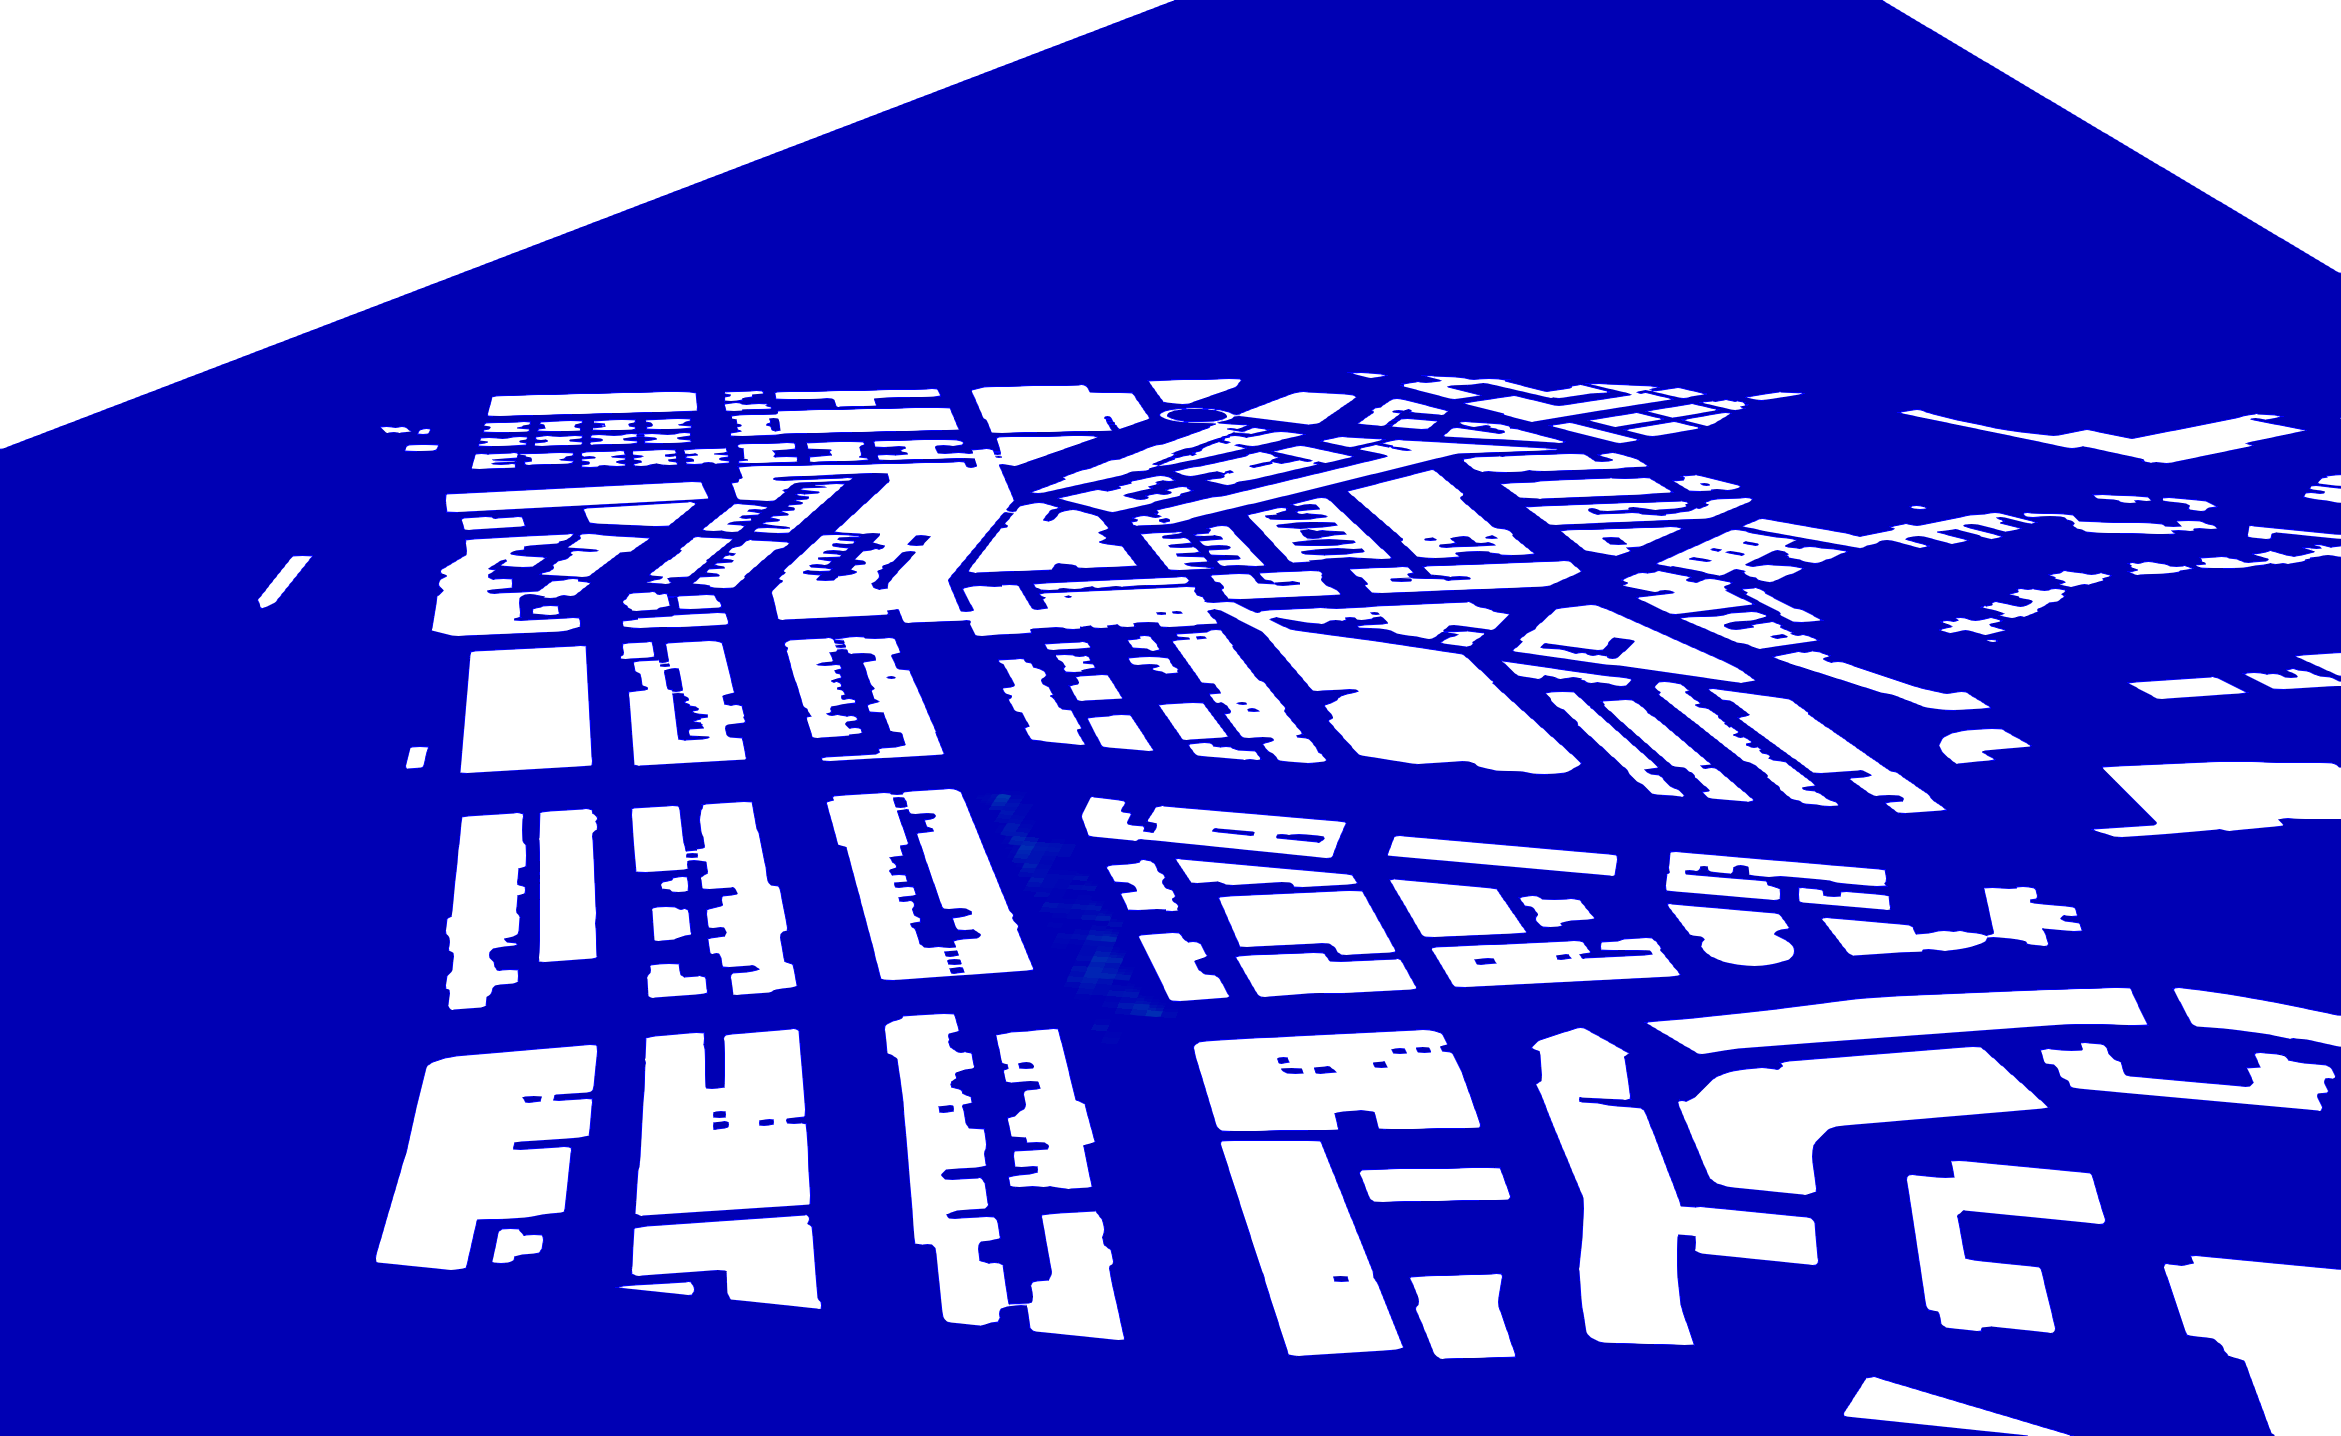
\includegraphics[width=0.23\textwidth, trim={500px 50px 1000px 200px},clip]{01_images/anim2/animV1.0002.png}};
        \node (right) at (left.east) [anchor=west] {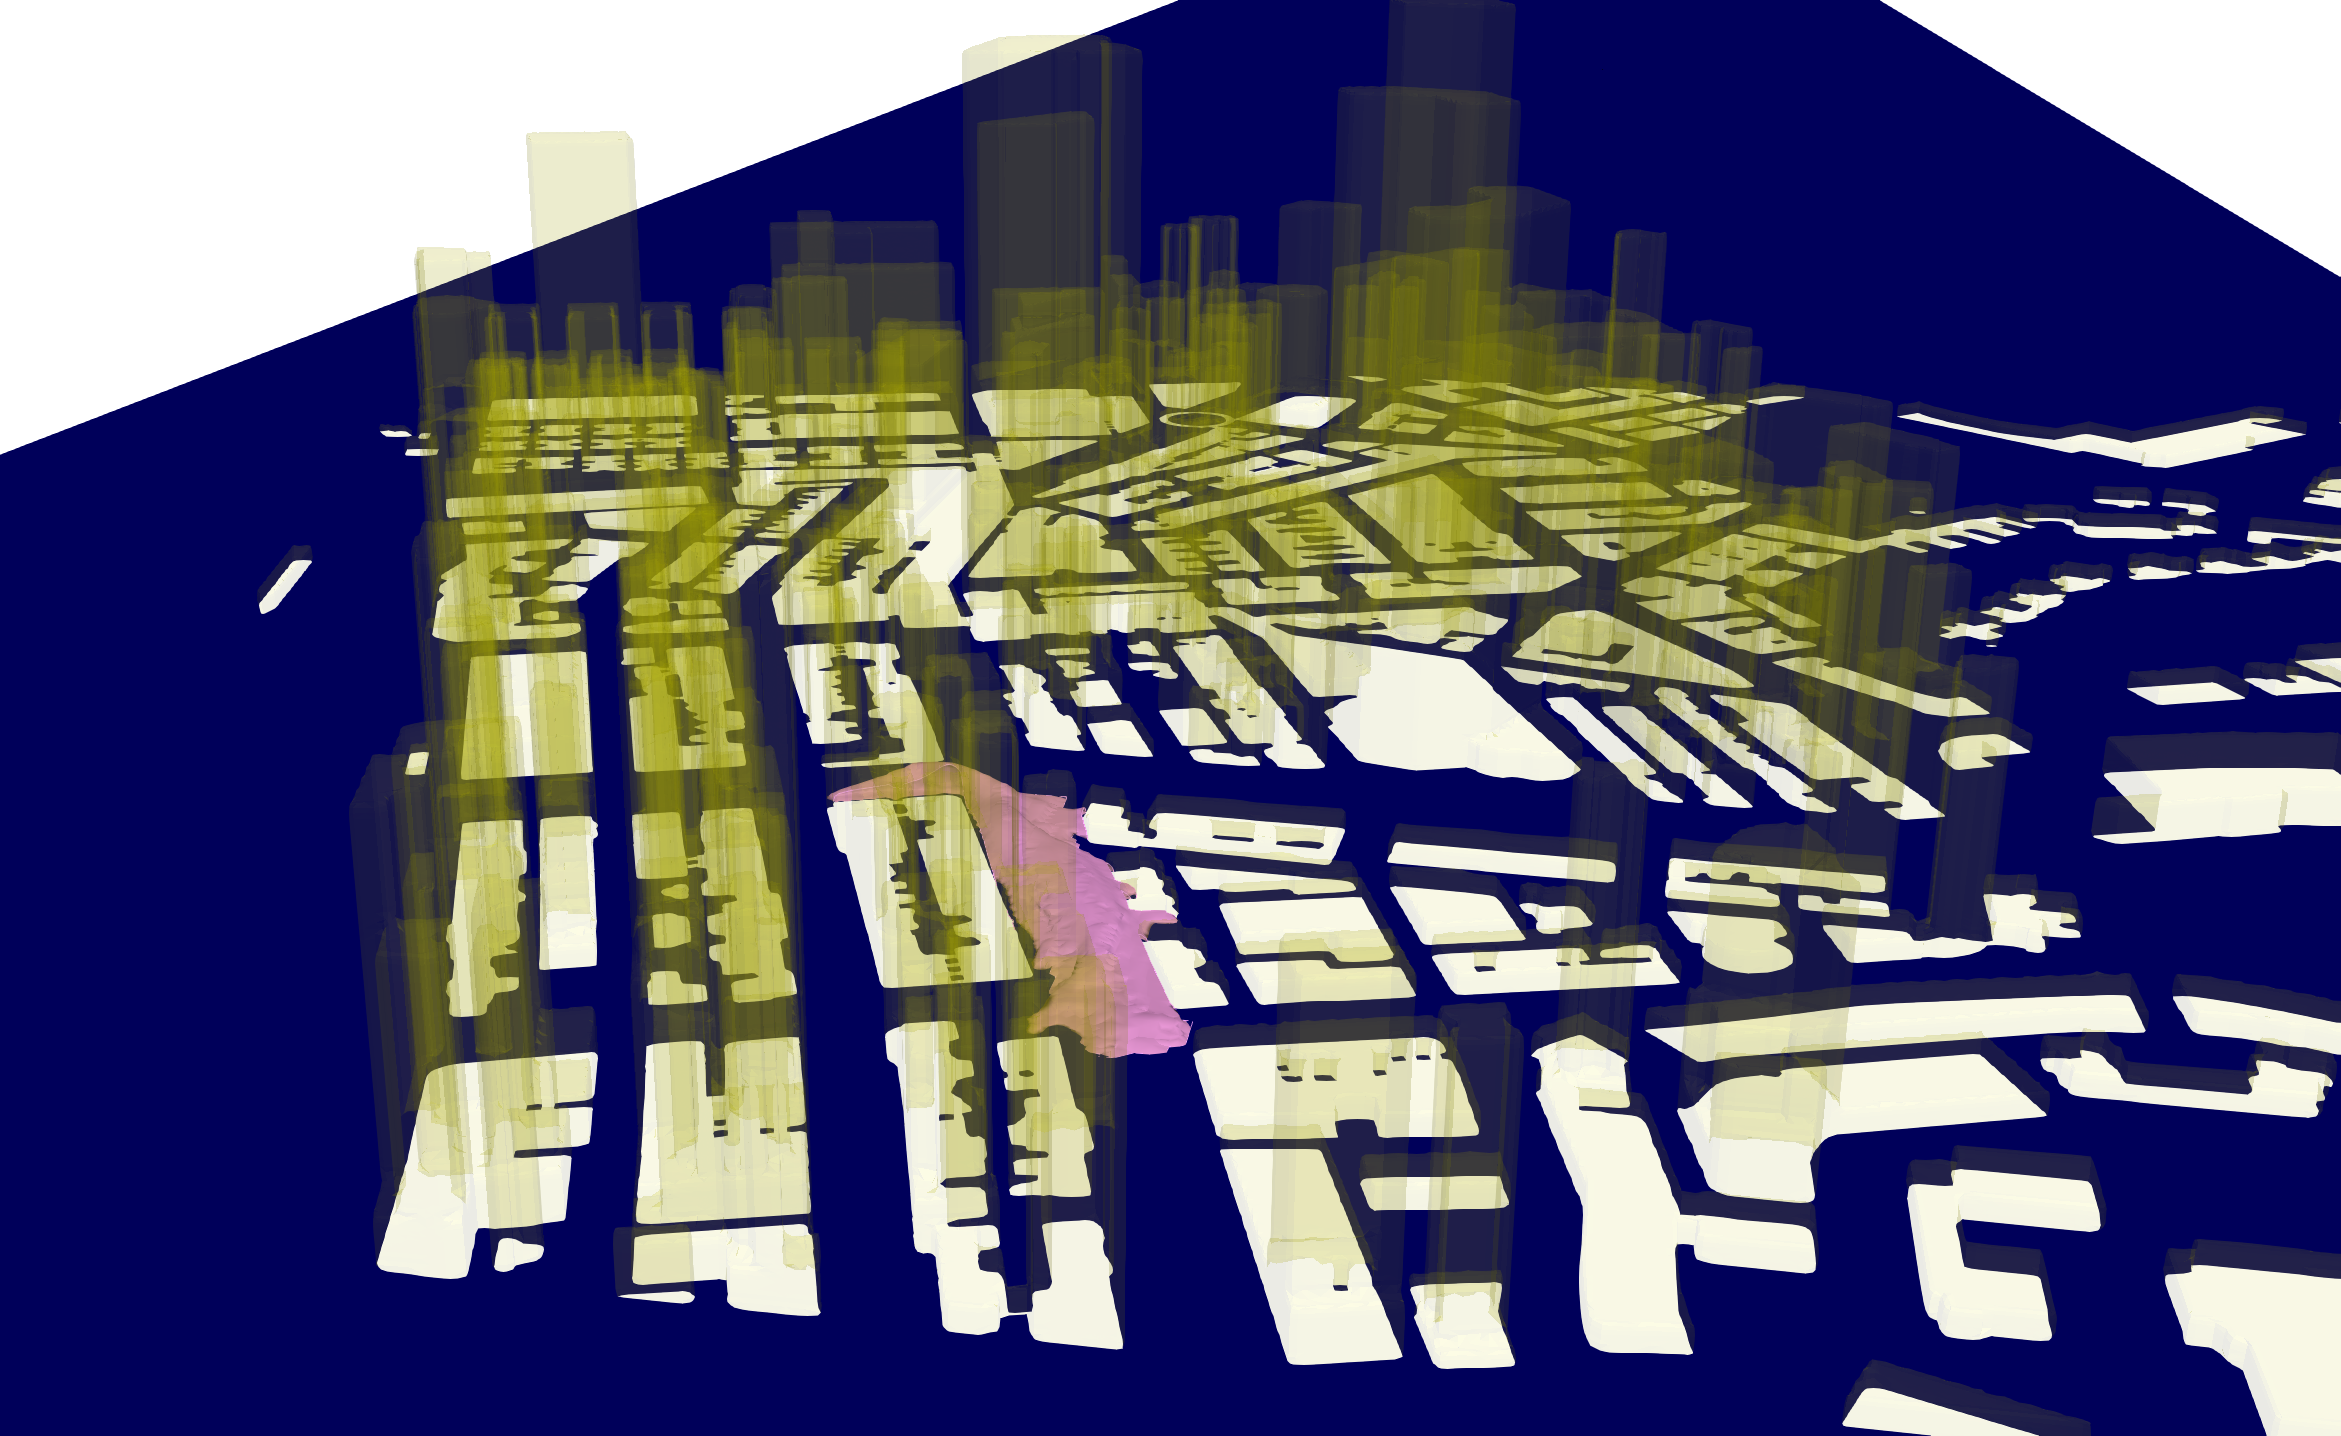
\includegraphics[width = 0.5\textwidth, trim={0 50px 0 200px},clip]{01_images/anim/animV1.0003.png}};
        \node at (right.west) [anchor=north, xshift = 0.2cm, rotate=90, color=white] {$t$ = 10\,s};
        \node (left) at (left.south) [anchor=north] {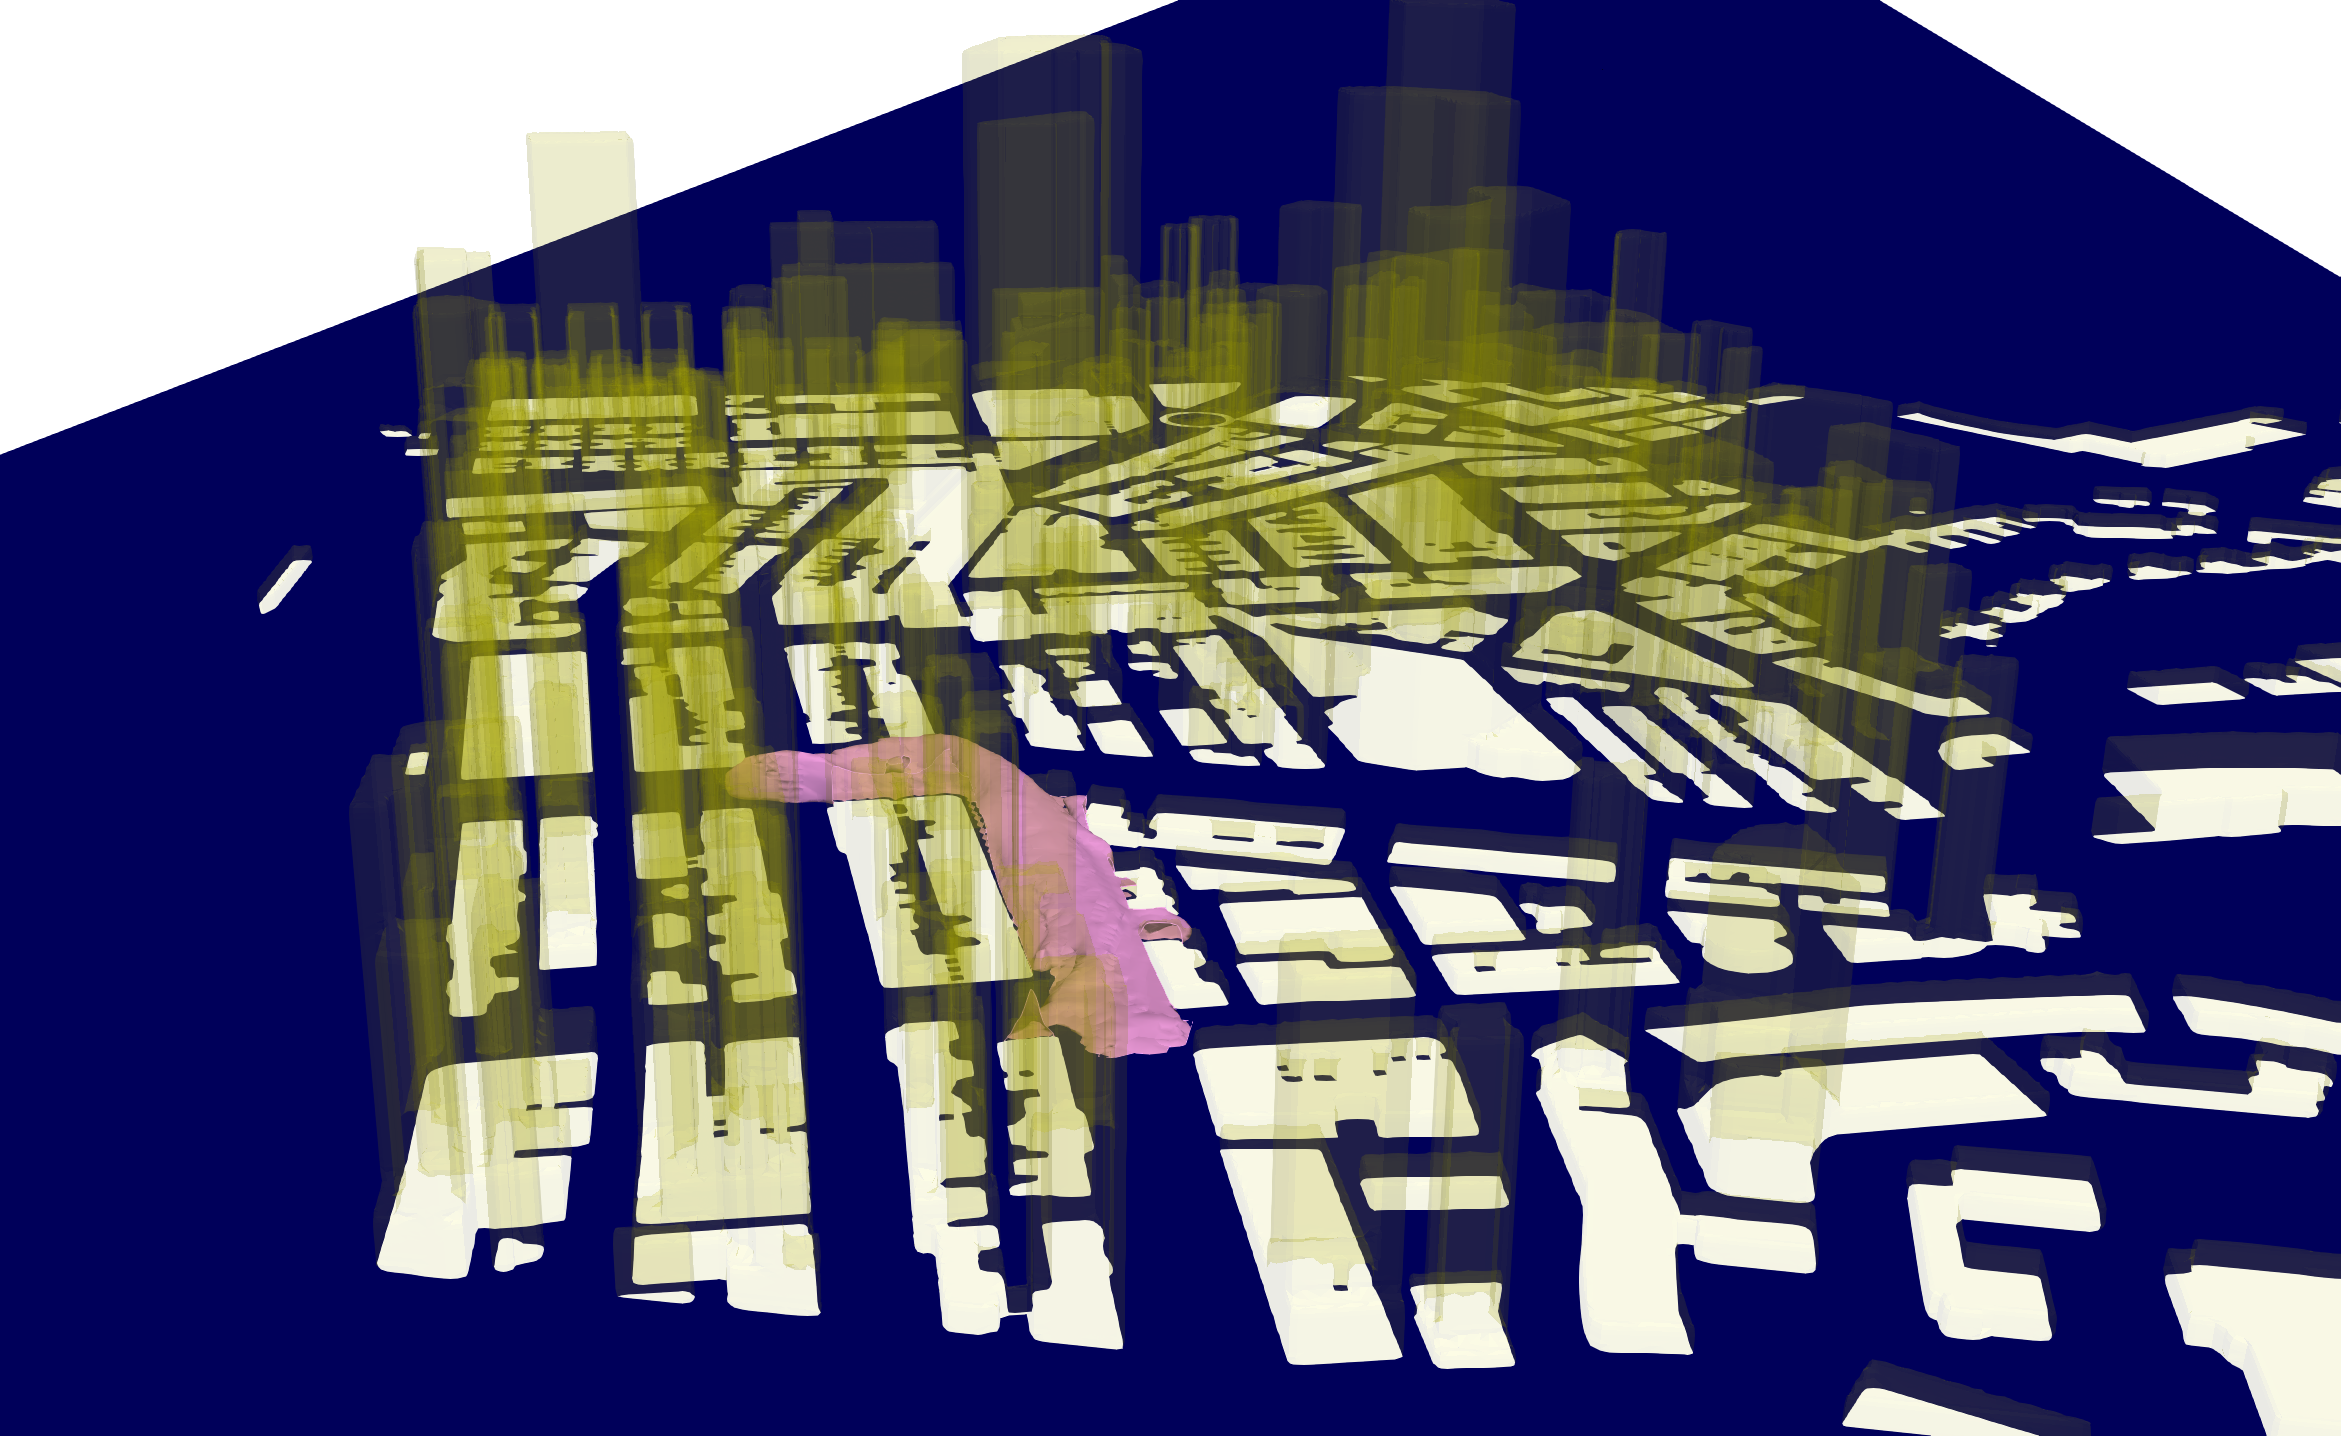
\includegraphics[width = 0.5\textwidth, trim={0 50px 0 200px},clip]{01_images/anim/animV1.0004.png}};
        \node at (left.west) [anchor=north, xshift = 0.2cm, rotate=90, color=white] {$t$ = 20\,s};
        \node (right) at (left.east) [anchor=west] {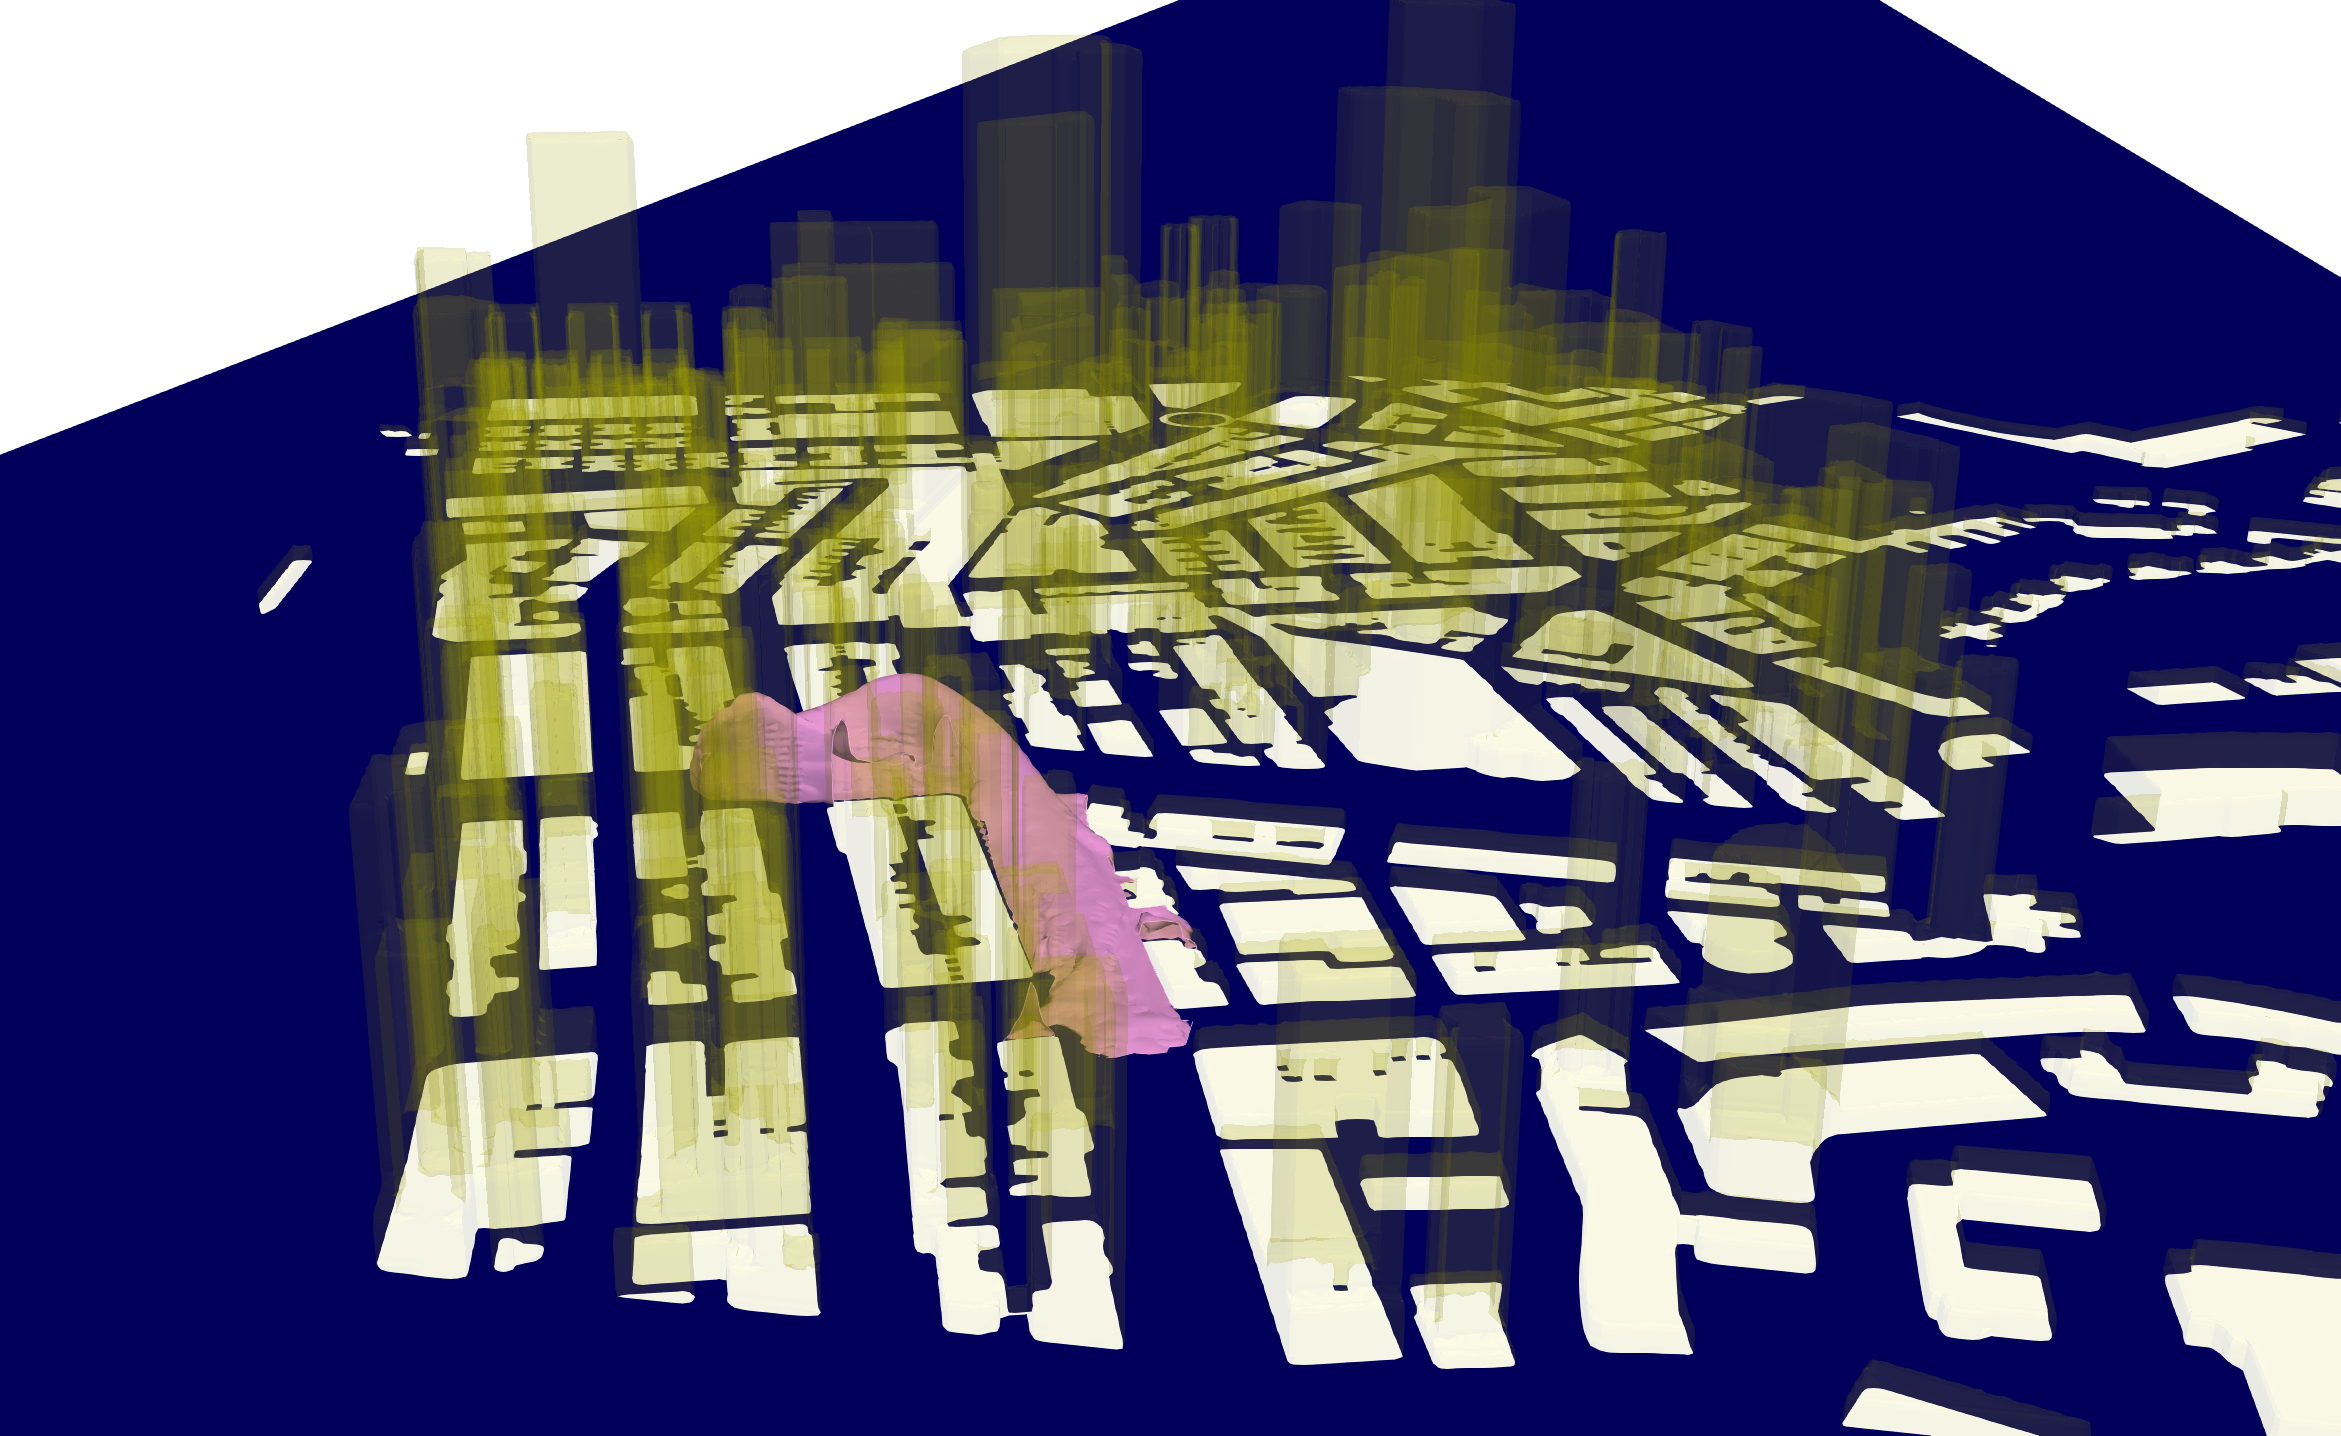
\includegraphics[width = 0.5\textwidth, trim={0 50px 0 200px},clip]{01_images/anim/animV1.0005.png}};
        \node at (right.west) [anchor=north, xshift = 0.2cm, rotate=90, color=white] {$t$ = 30\,s};
        % \node (right) at (left.east) [anchor=west] {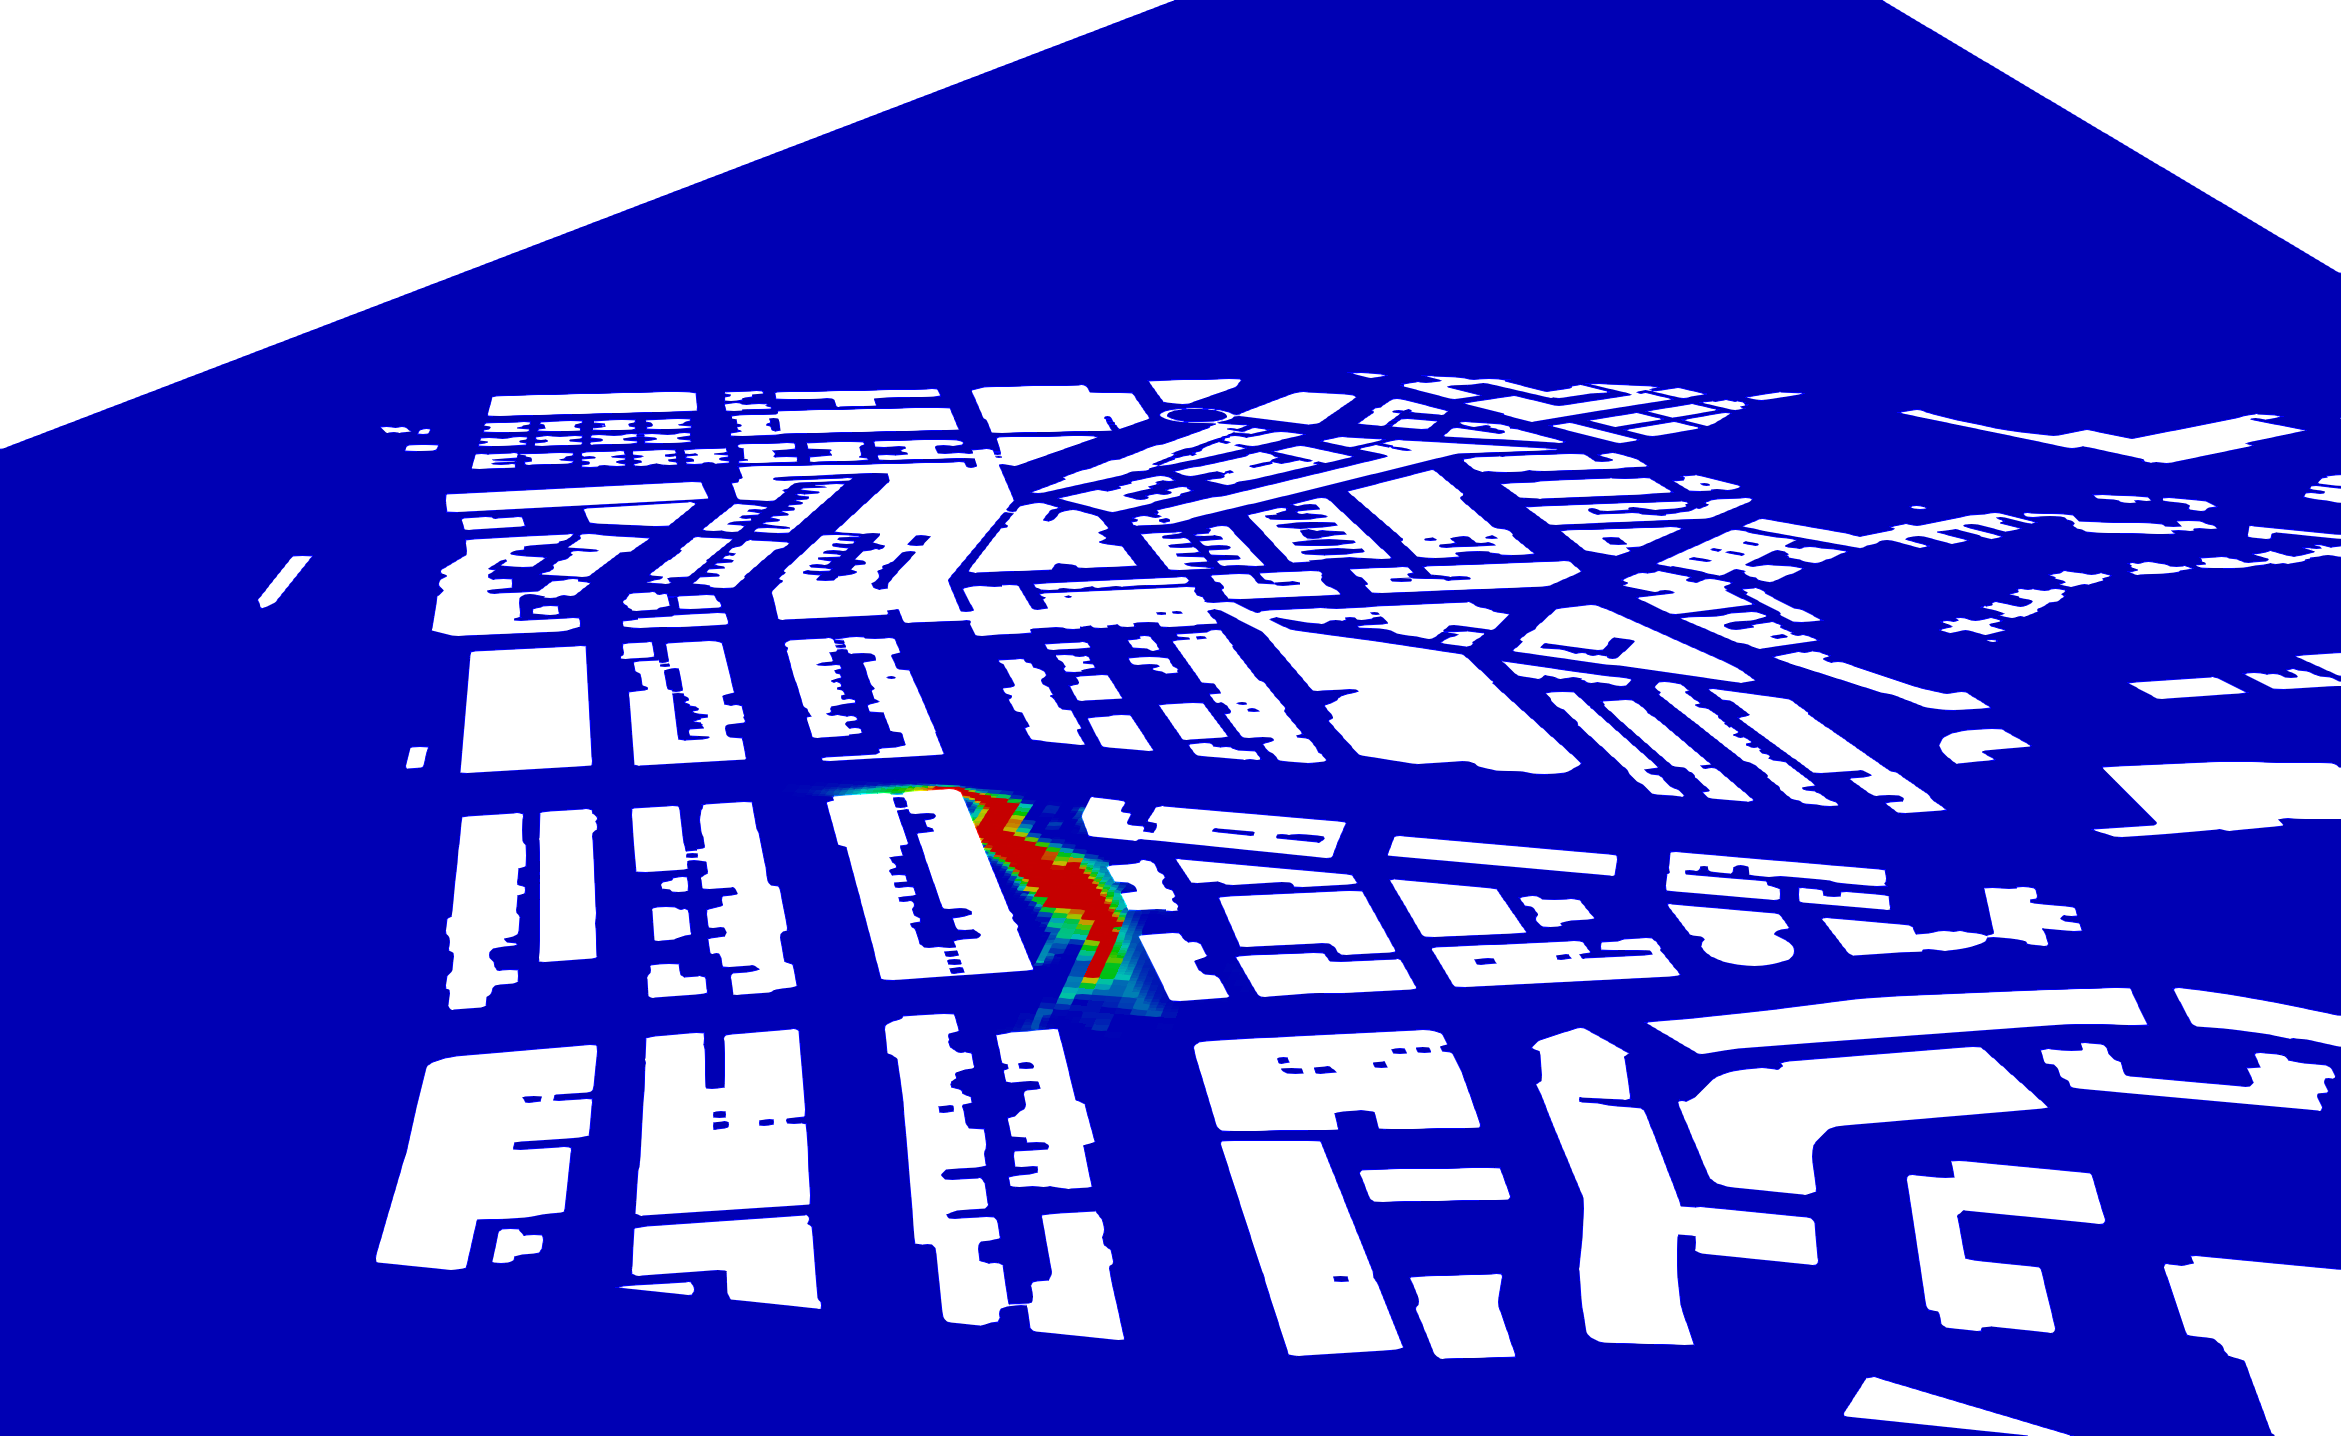
\includegraphics[width=0.23\textwidth, trim={500px 50px 1000px 200px},clip]{01_images/anim2/animV1.0003.png}};
        \node (left) at (left.south) [anchor=north] {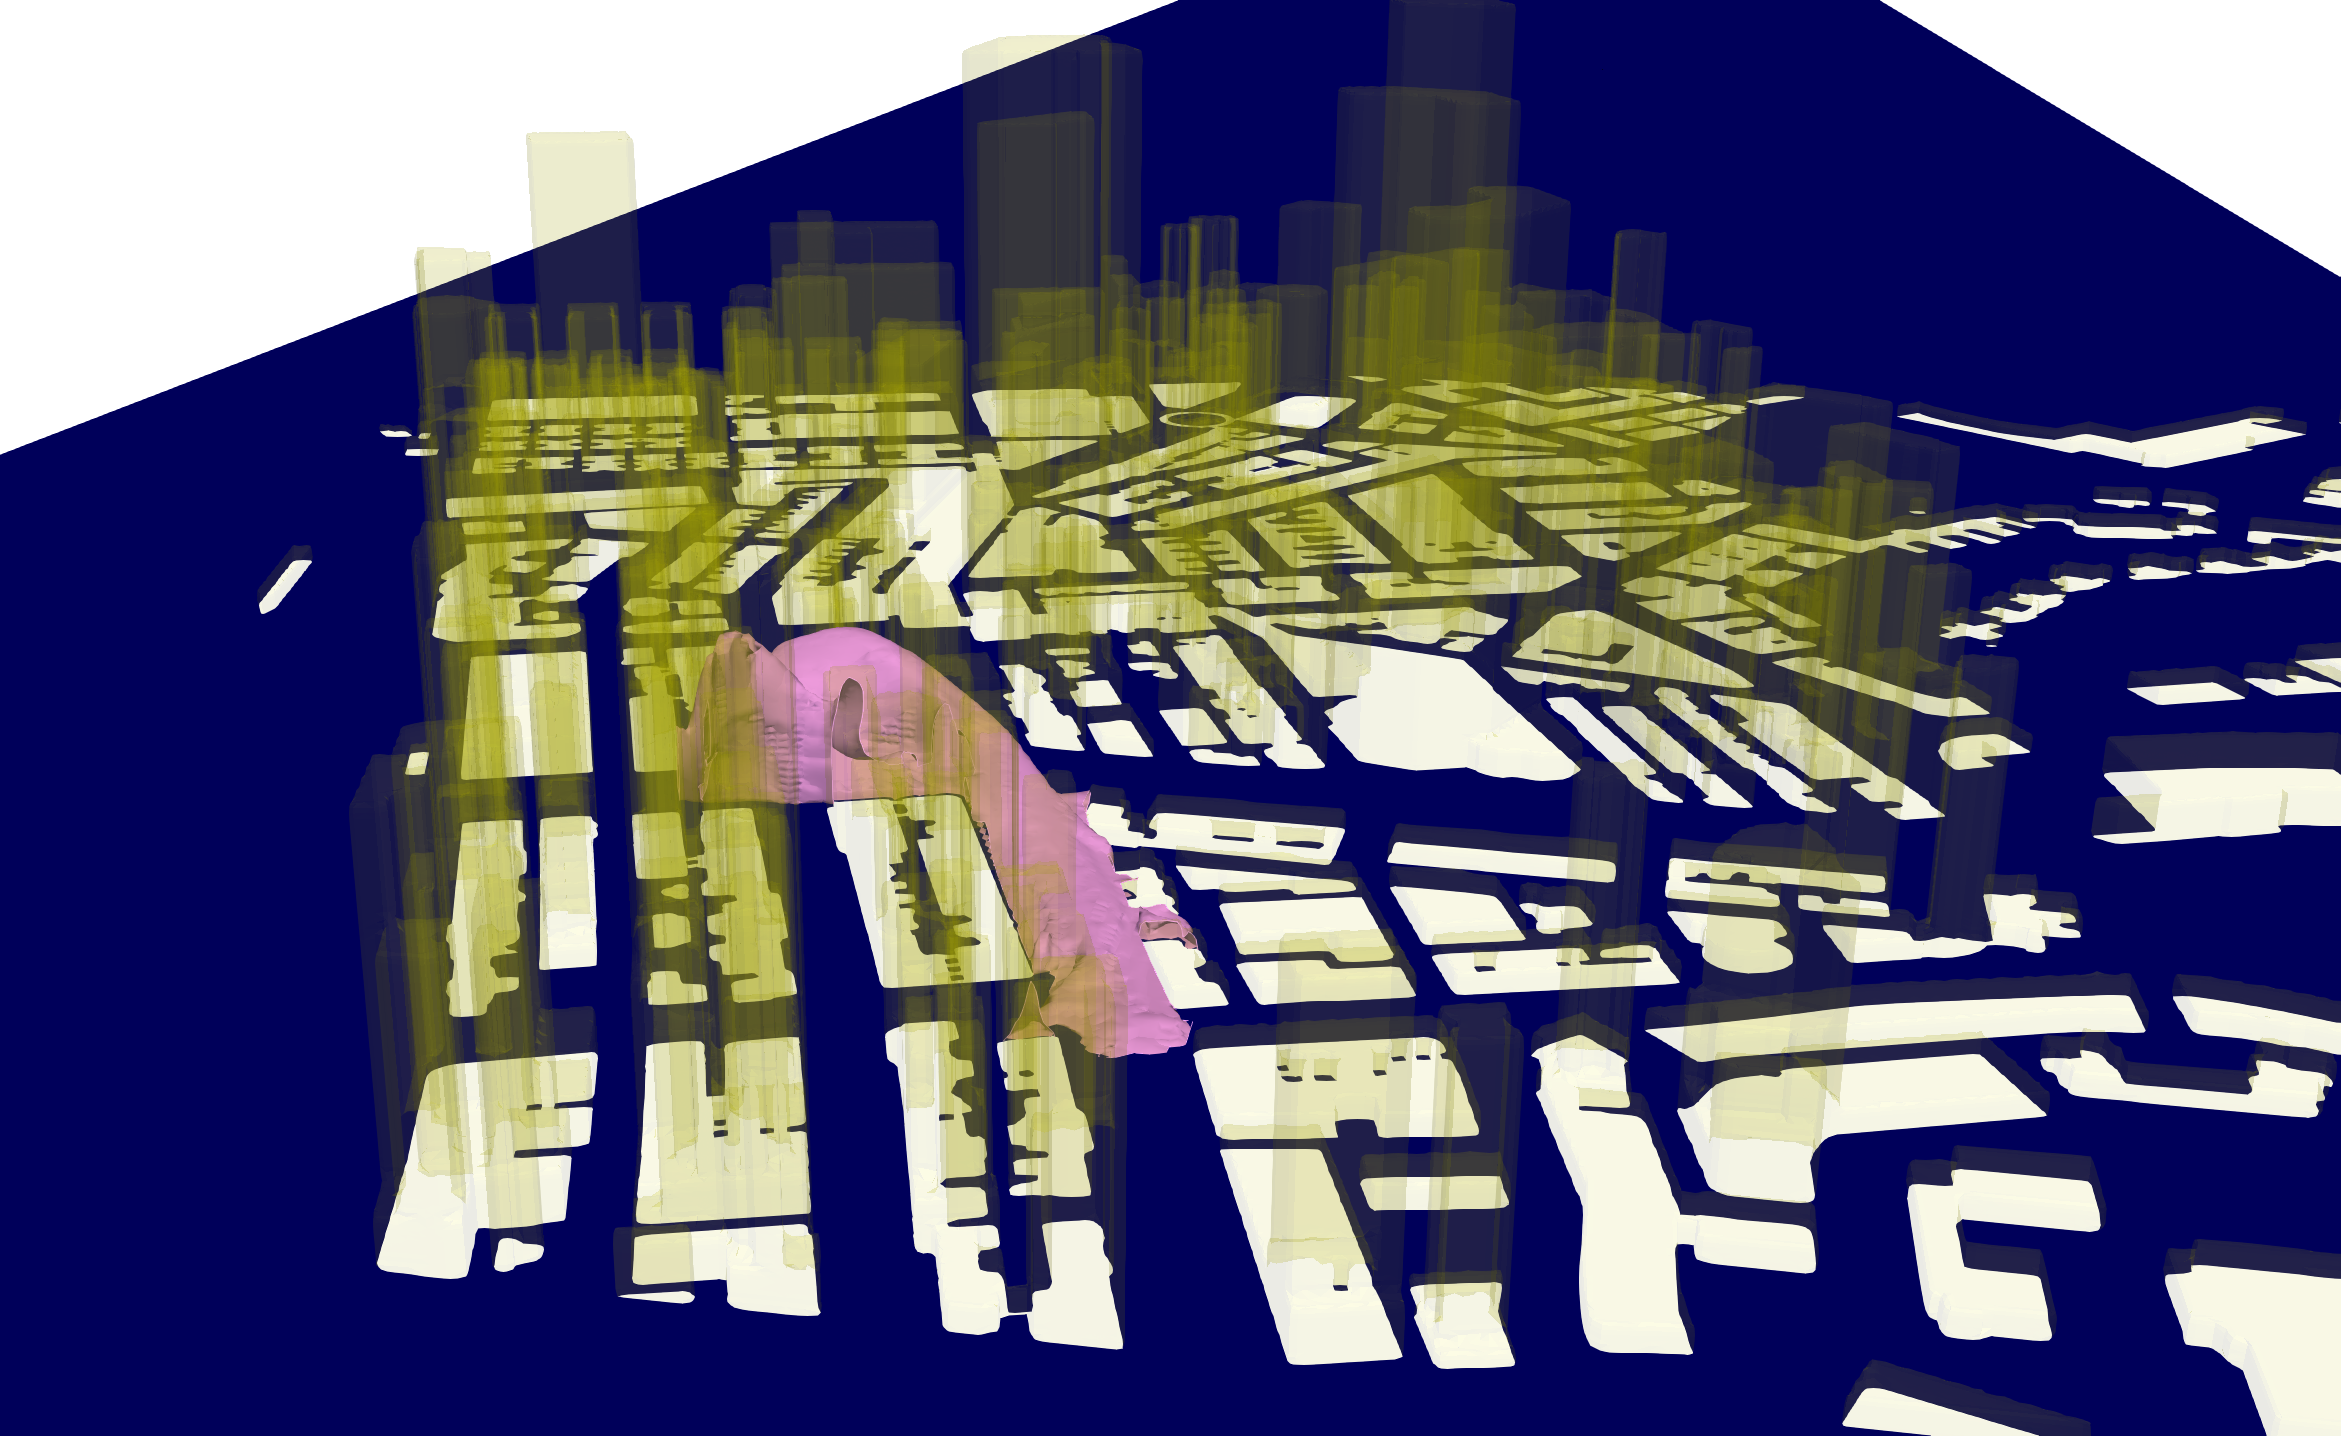
\includegraphics[width = 0.5\textwidth, trim={0 50px 0 200px},clip]{01_images/anim/animV1.0006.png}};
        \node at (left.west) [anchor=north, xshift = 0.2cm, rotate=90, color=white] {$t$ = 40\,s};
        \node (right) at (left.east) [anchor=west] {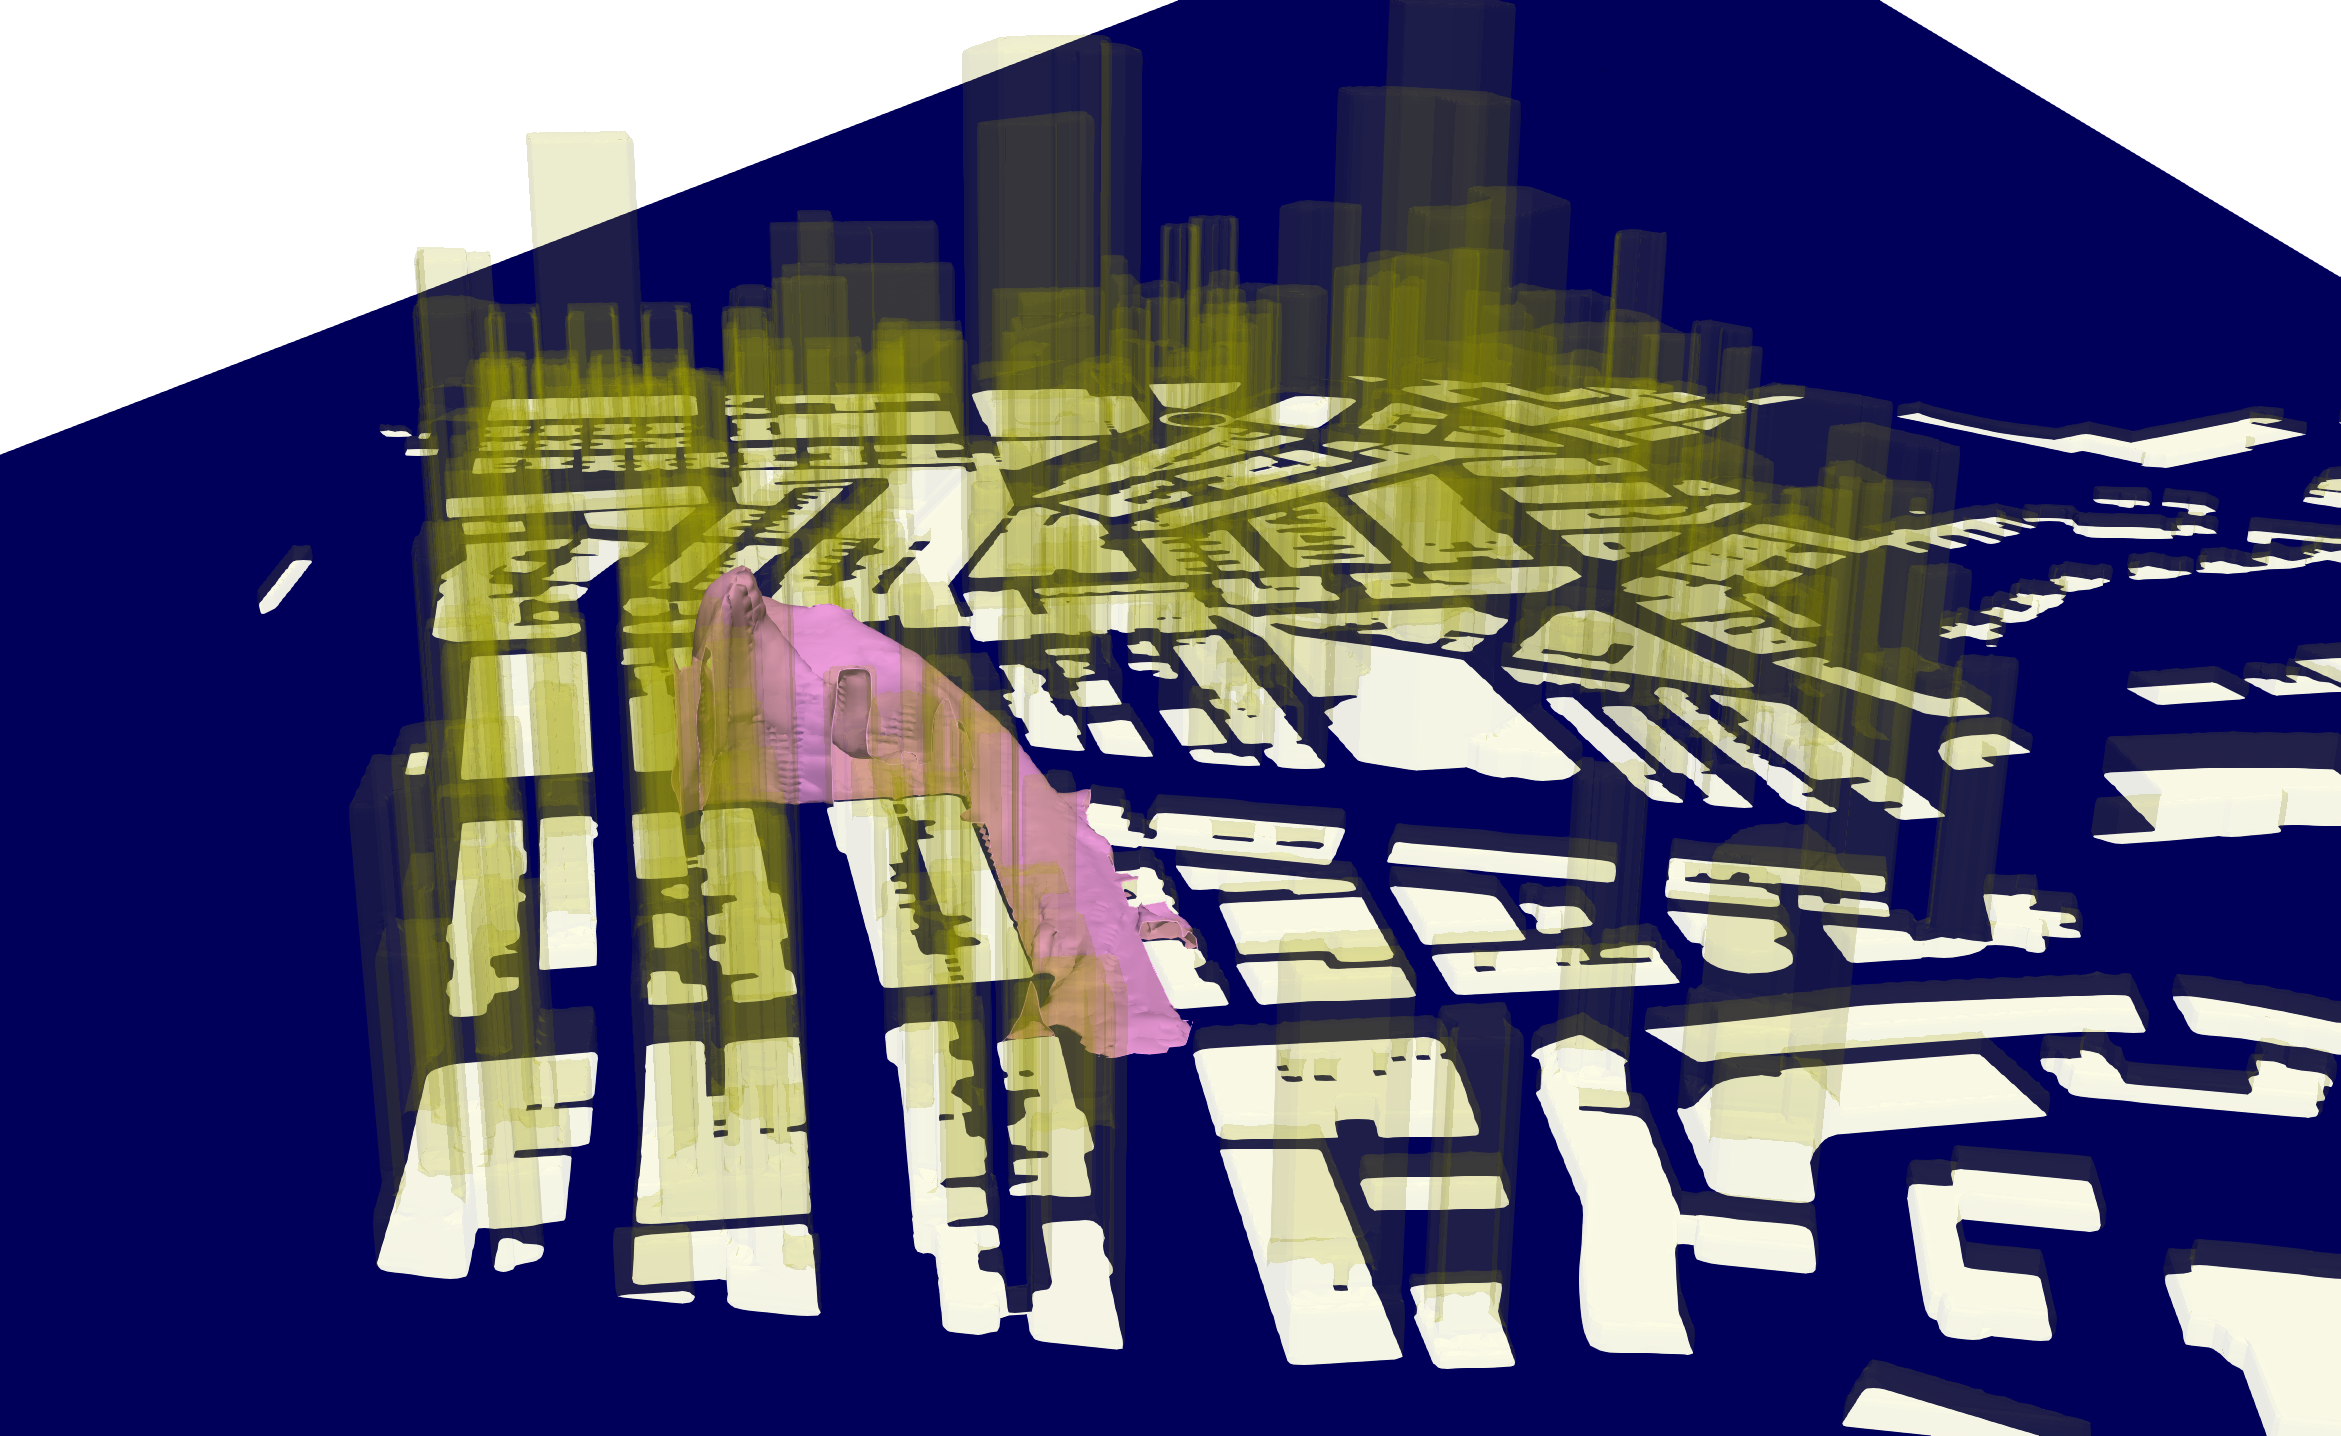
\includegraphics[width = 0.5\textwidth, trim={0 50px 0 200px},clip]{01_images/anim/animV1.0007.png}};
        \node at (right.west) [anchor=north, xshift = 0.2cm, rotate=90, color=white] {$t$ = 50\,s};
        % \node (right) at (left.east) [anchor=west] {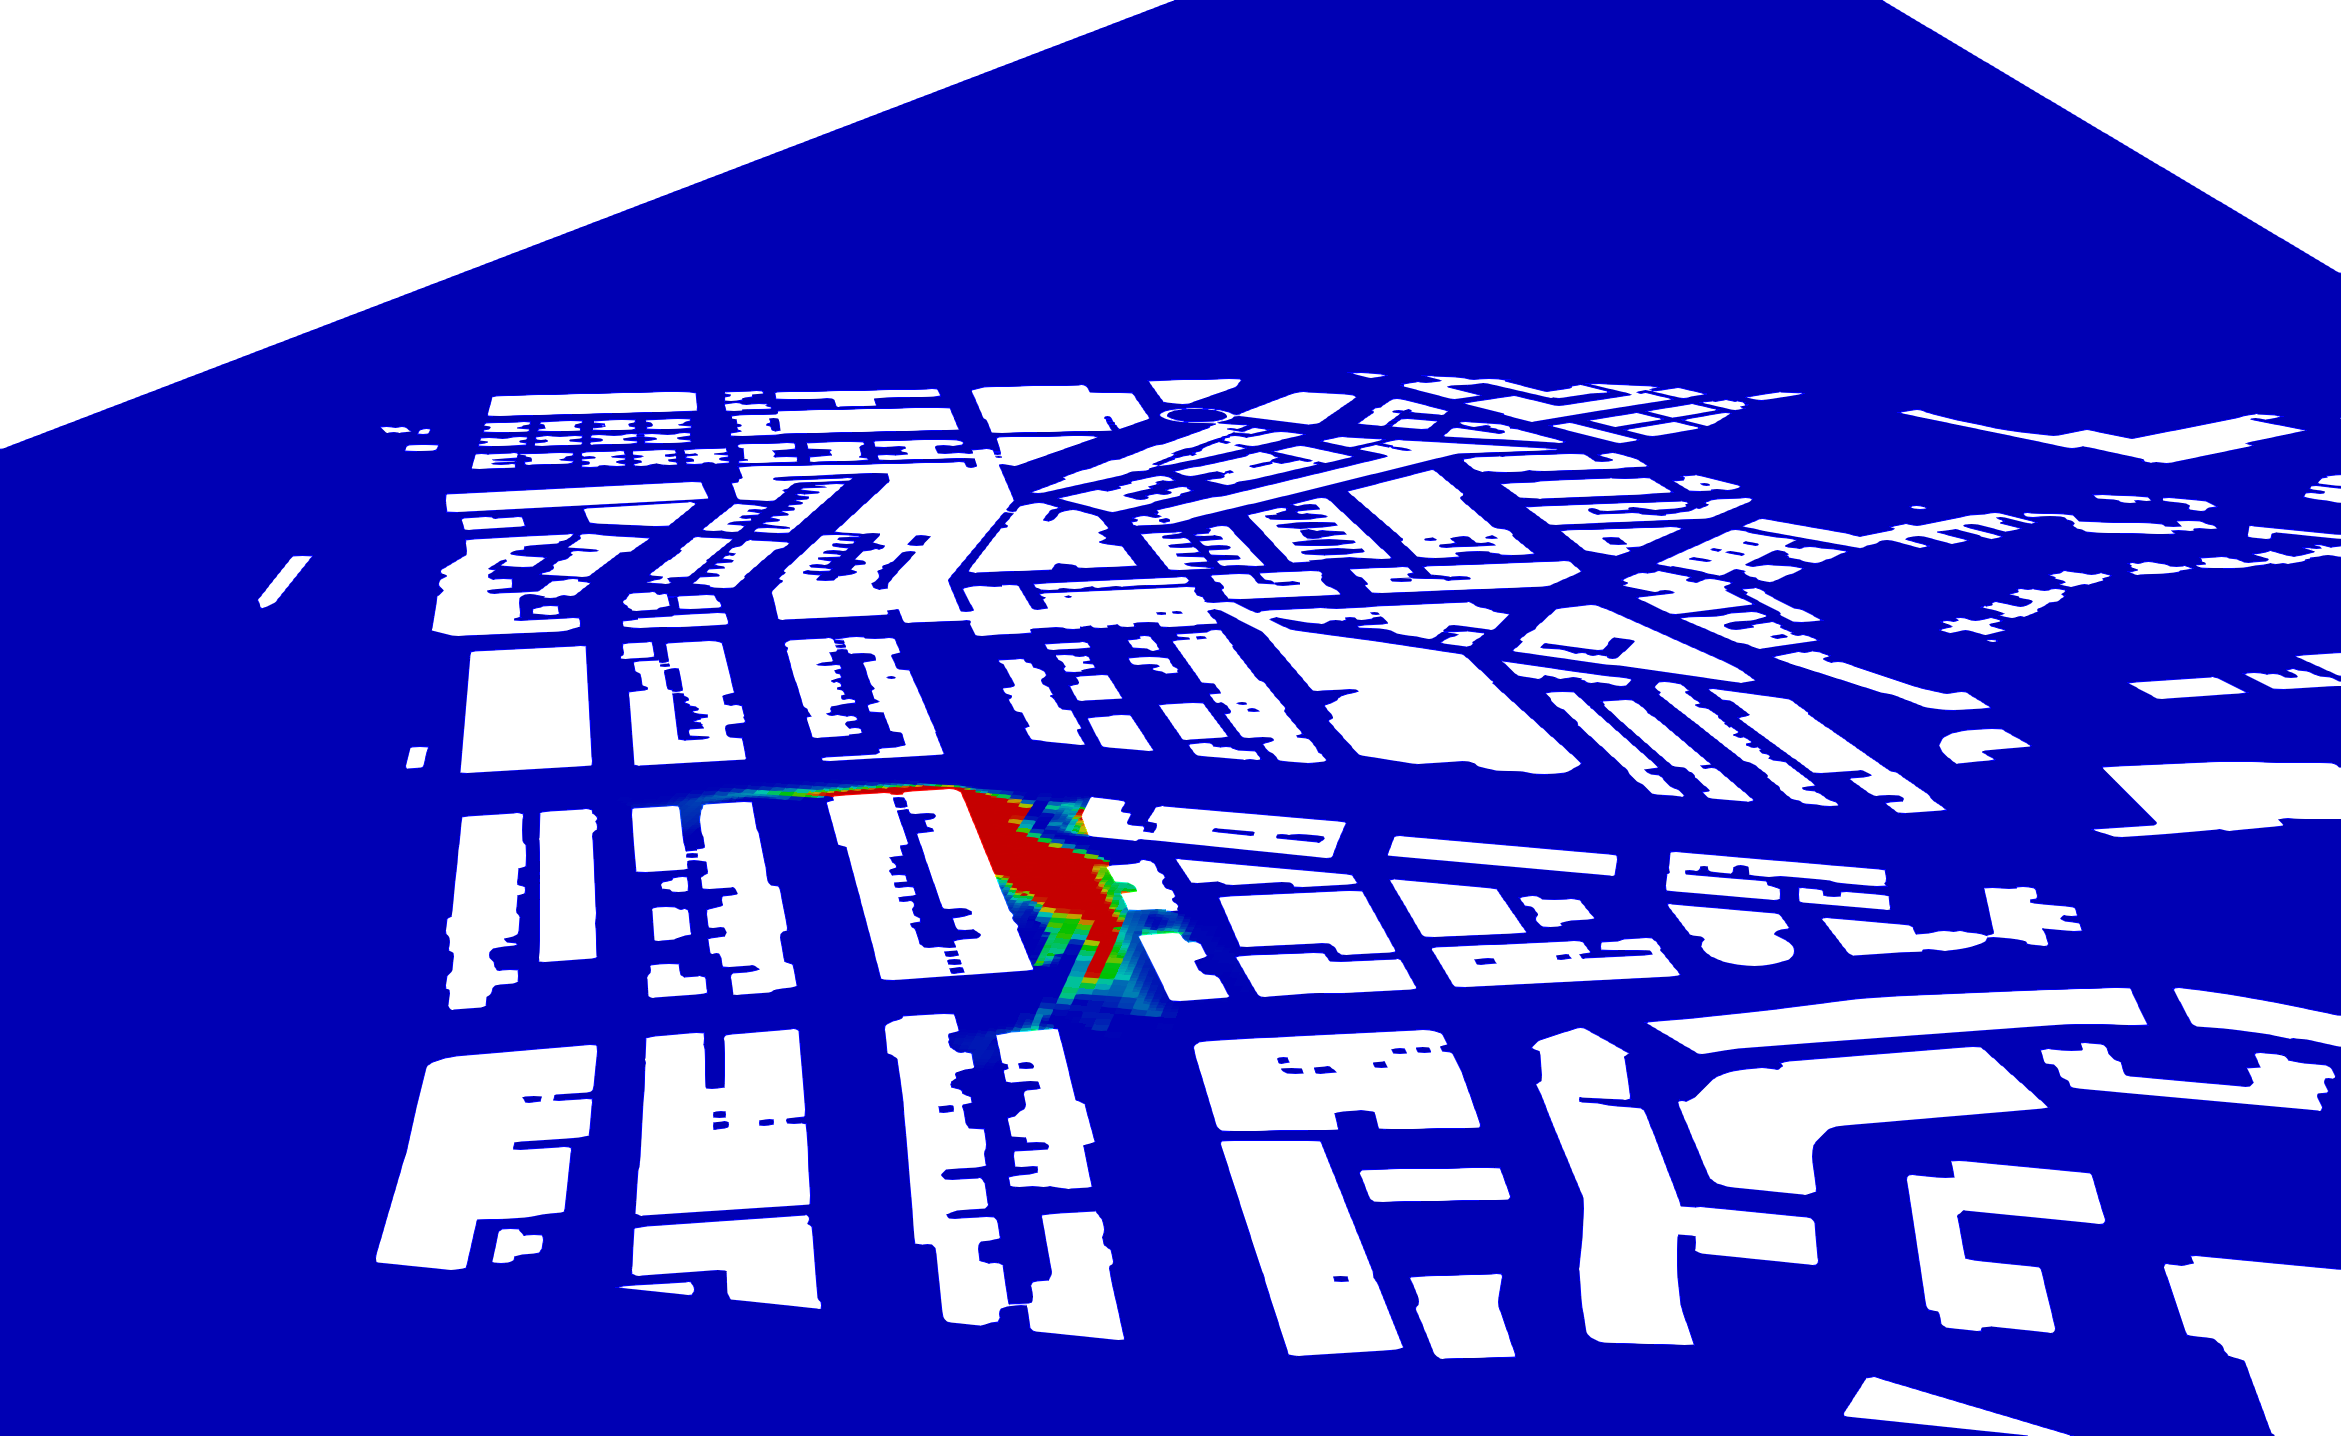
\includegraphics[width=0.23\textwidth, trim={500px 50px 1000px 200px},clip]{01_images/anim2/animV1.0005.png}};
        \node (left) at (left.south) [anchor=north] {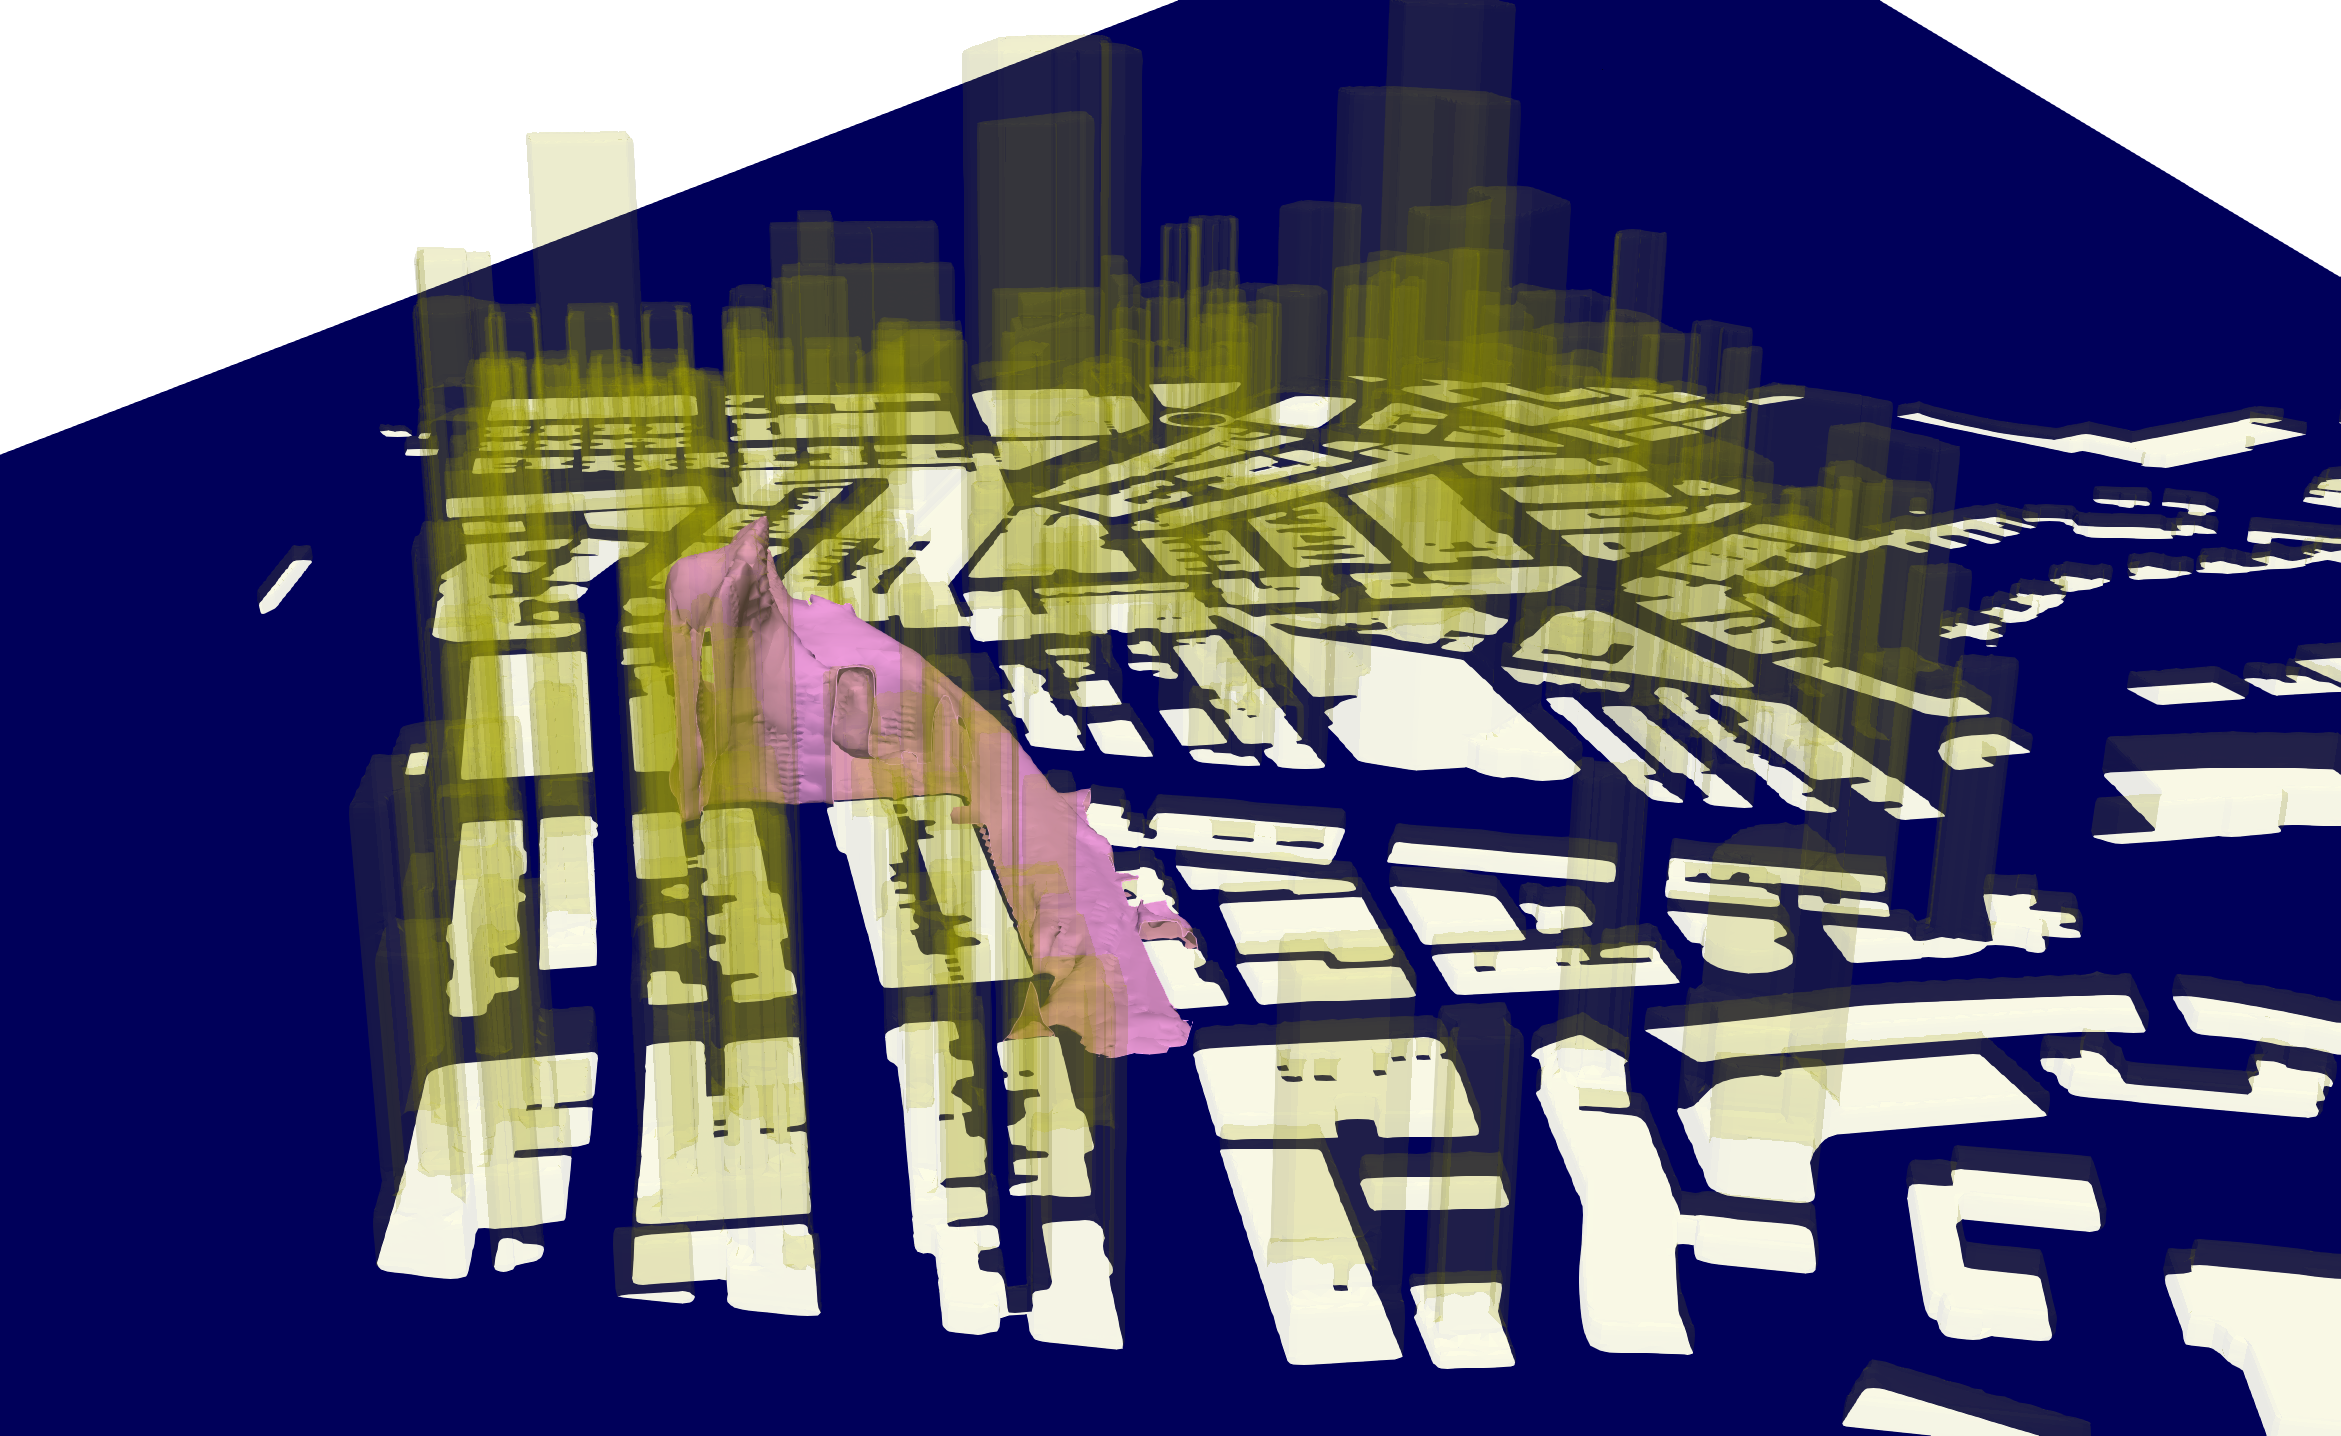
\includegraphics[width = 0.5\textwidth, trim={0 50px 0 200px},clip]{01_images/anim/animV1.0008.png}};
        \node at (left.west) [anchor=north, xshift = 0.2cm, rotate=90, color=white] {$t$ = 60\,s};
        \node (right) at (left.east) [anchor=west] {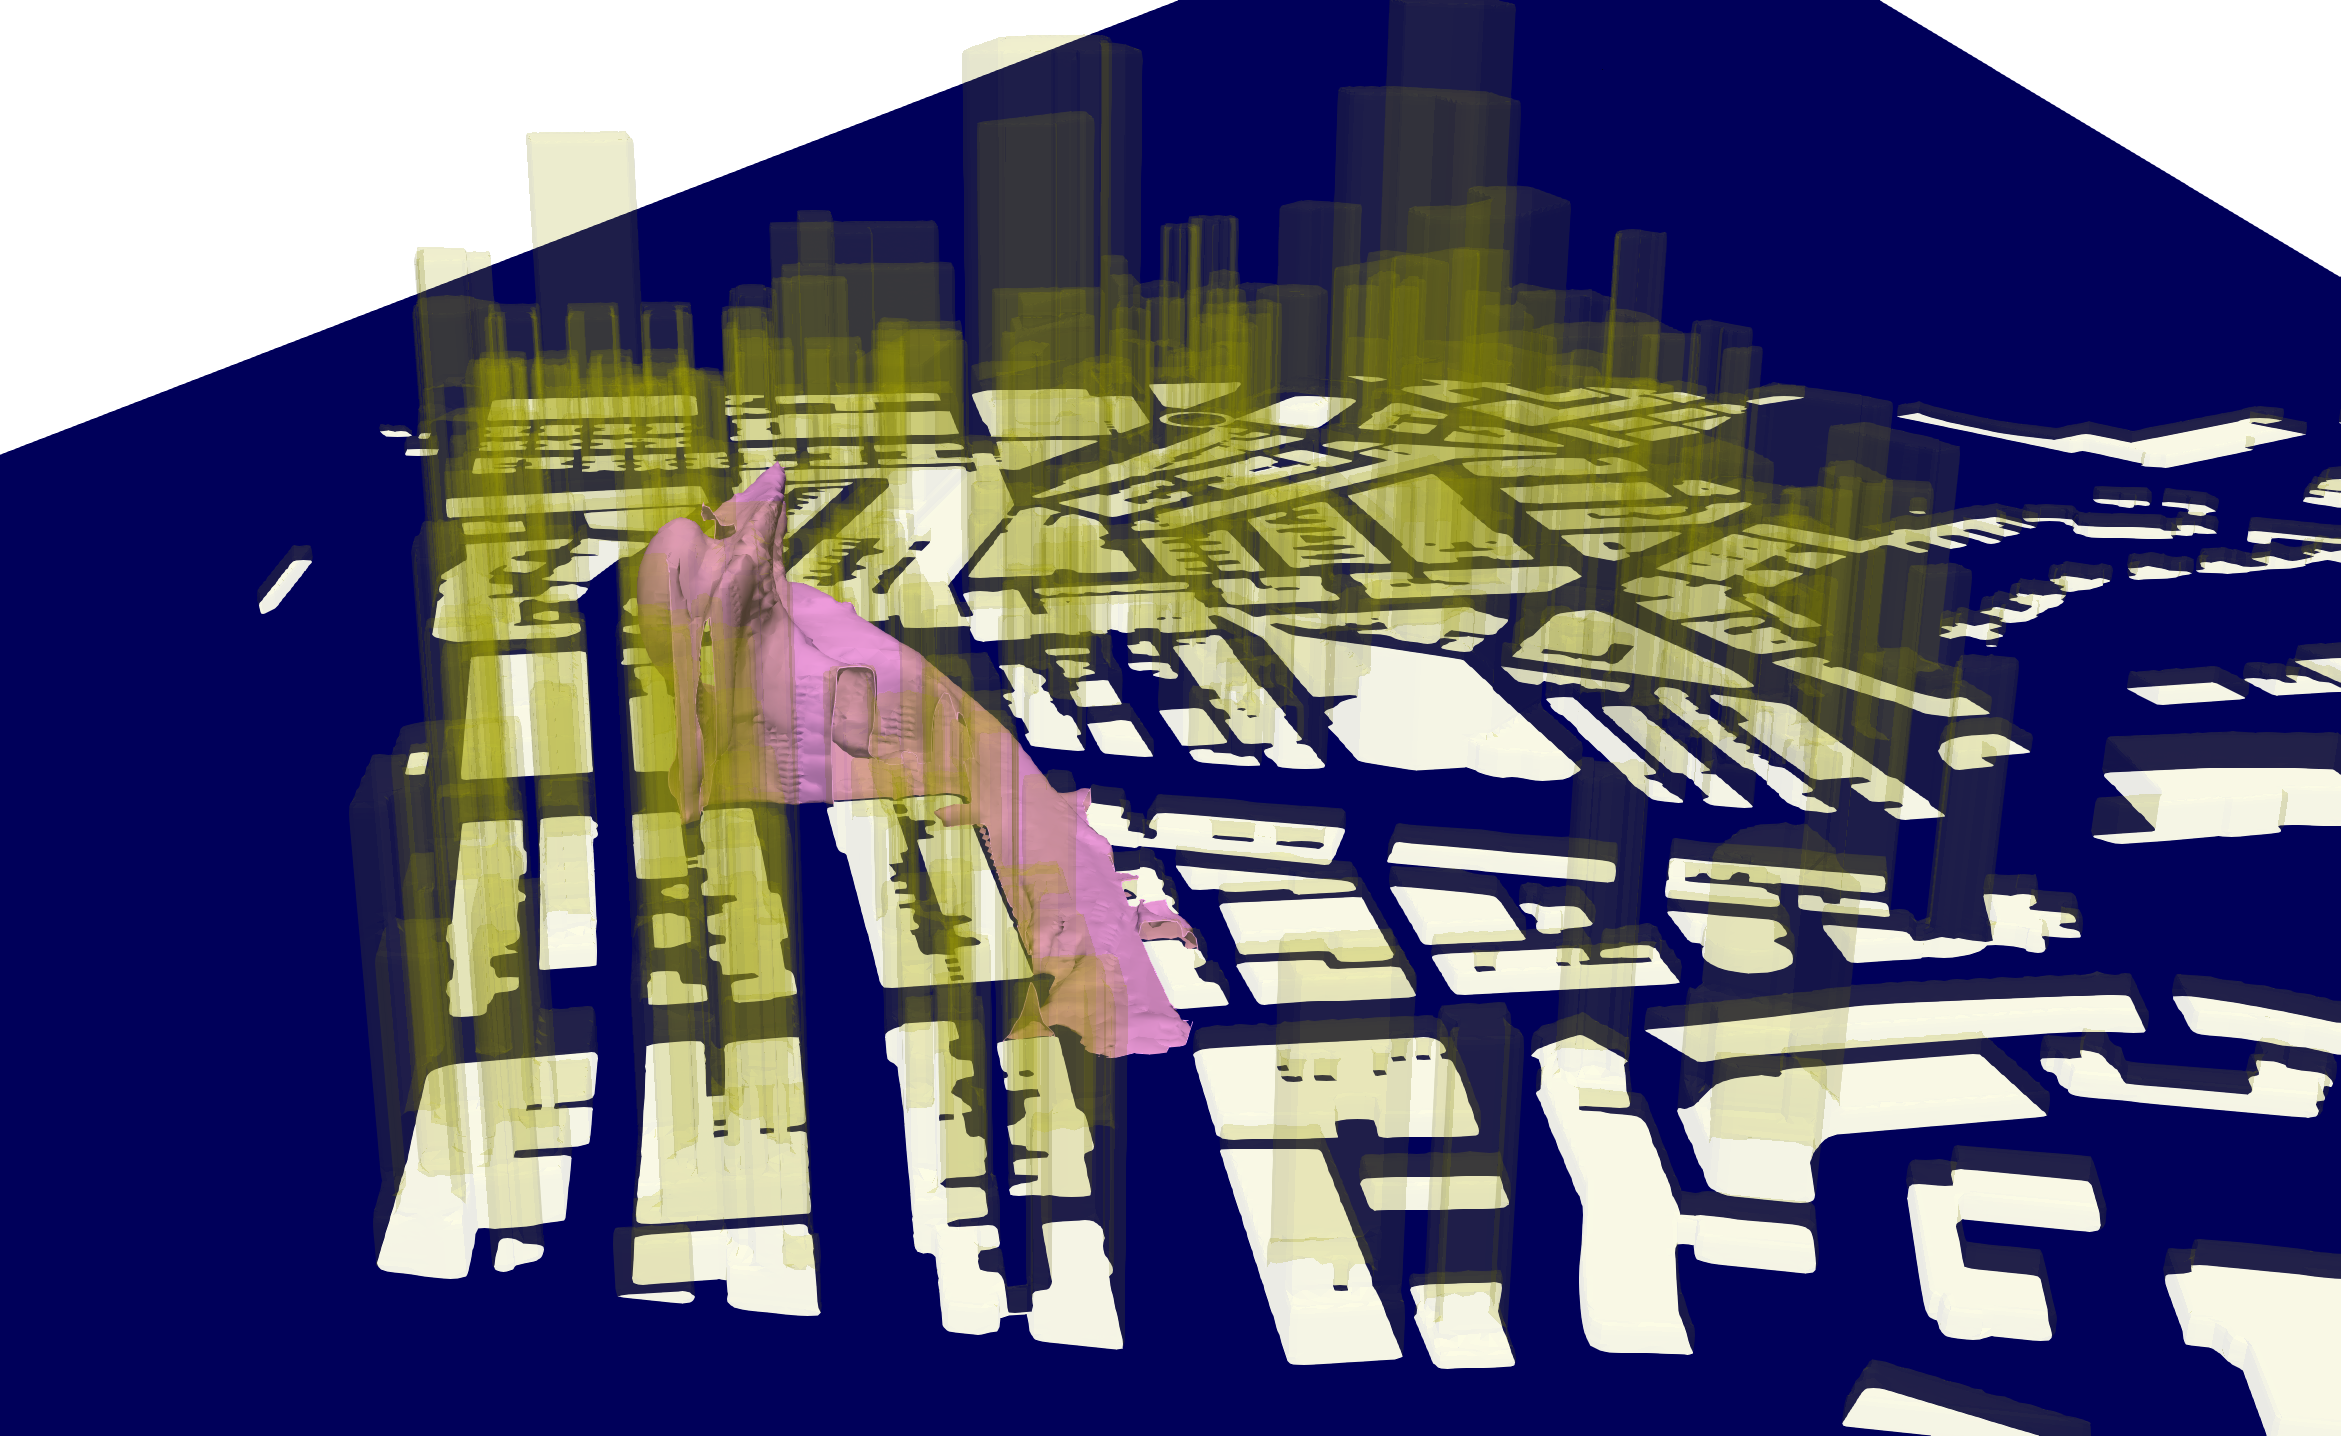
\includegraphics[width = 0.5\textwidth, trim={0 50px 0 200px},clip]{01_images/anim/animV1.0009.png}};
        \node at (right.west) [anchor=north, xshift = 0.2cm, rotate=90, color=white] {$t$ = 70\,s};
        % \node (right) at (left.east) [anchor=west] {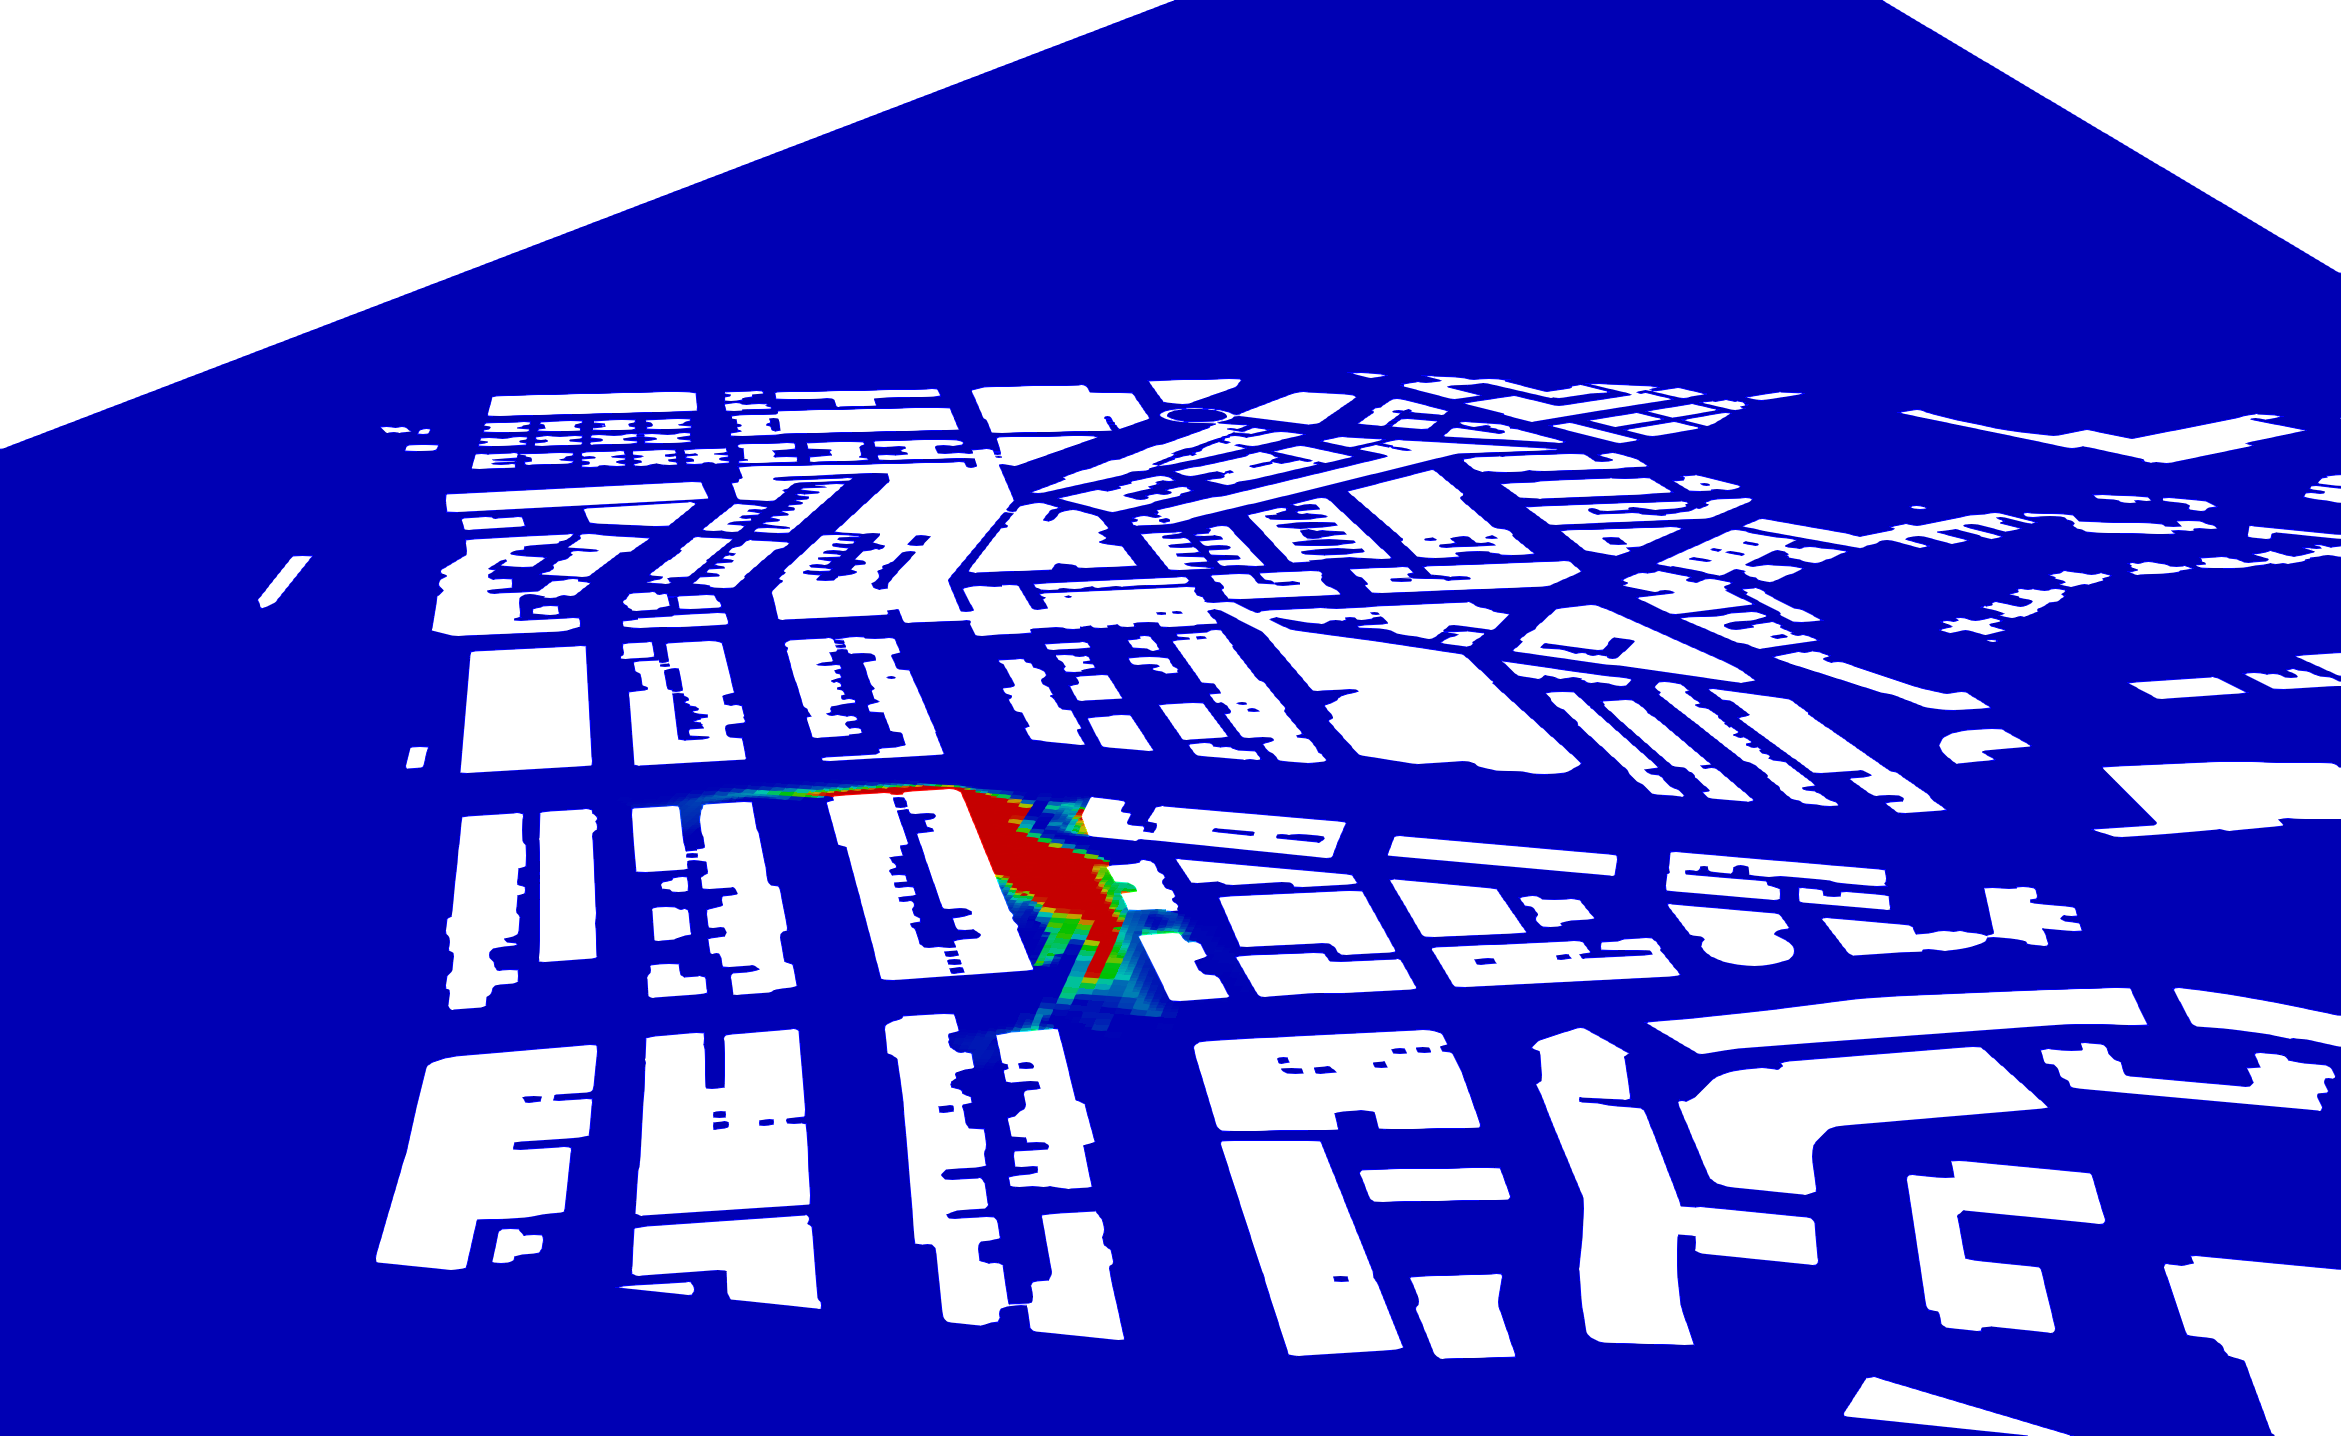
\includegraphics[width=0.23\textwidth, trim={500px 50px 1000px 200px},clip]{01_images/anim2/animV1.0005.png}};
    \end{tikzpicture}
    \caption{Time development of the air pollution spreading inside city, contour $y_{\mathrm{pol}}\,=\,1\,$ppm in pink.}
    \label{fig:pol}
\end{figure}

Next, main flow pathways are visualized utilizing the flow streamlines colored by the streamwise velocity component in Figure~\ref{fig:ux_p}b.

Steady-state velocity field obtained by the solution of~(\ref{eq:RANS1},~\ref{eq:RANS2}) can be used in the simulation of the pollution spreading, which is assumed transient. The resulting time development of the pollution at street is visualized by $y_{\mathrm{pol}}\,=\,1\,$ppm contour colored by pink in Figure~\ref{fig:pol} for times $t\,=\,$1, 10, 20, 30, 40, 50, 60, and 70\,s.
\cleardoublepage
\section{Conclusions}
\label{sec:concl}

\noteTH{And conclusion here}
\cleardoublepage
\section{Nomenclature}

\begin{longtable}{lp{0.1\textwidth}l}
    $c_i$ & \dotfill & Molar concentration of $i$-th molar specie\\
    $c_{\mathrm{T}}$ & \dotfill & Total molar concentration\\
    $\Co$ & \dotfill & Courant number\\
    $d$ & \dotfill & Diameter\\
    $D_i$ & \dotfill & Molar diffusivity of $i$-th molar specie\\
    $D_i^{\mathrm{eff}}$ & \dotfill & Effective molar diffusivity of $i$-th molar specie\\
    $\bm{d}_{\mathrm{PN}}$ & \dotfill & Vector connecting centroids of P and N\\
    $f$&\dotfill & Face of the cell\\
    $\bm{f}_b$&\dotfill & Body forces acting on cell\\
    $\bm{g}$ & \dotfill & Gravitational acceleration\\
    $h$ & \dotfill & Specific enthalpy\\
    $I$ & \dotfill & Time interval\\
    $I^h$ & \dotfill & Discretized time interval\\
    ${m}$&\dotfill & Number of discretized FV cells\\
    ${M}$&\dotfill & Molar mass\\
    ${n}$&\dotfill & Number of species\\
    $\bm{n}$&\dotfill & Outer normal vector\\
    $\bm{n}_f$&\dotfill & Outer normal vector of the face $f$\\
    ${p}$ &\dotfill & Pressure\\
    ${p_{\mathrm{ref}}}$ &\dotfill & Reference pressure\\
    $\tilde{p}$ & \dotfill & Kinematic pressure\\
    $Q$ & \dotfill & Computational domain\\
    $r_i$ & \dotfill & Reaction source of the $i$-th molar specie\\
    $\mathrm{R^g}$ & \dotfill & Universal gas constant\\
    $\Rey$ & \dotfill & Reynolds number\\
    ${s}_{\phi}$ &\dotfill & Source of the $\phi$\\
    $\bm{S}_{f}$ & \dotfill & Face area vector\\
    $t$ &\dotfill & Time\\
    $T$ &\dotfill & Temperature\\
    ${T_{\mathrm{ref}}}$ &\dotfill & Reference temperature\\
    $\bm{u} = (u,v,w)$&\dotfill & Velocity\\
    $y_i$&\dotfill & Molar fraction of the $i$-molar specie\\
    $\alpha$  &\dotfill & Heat transfer coefficient\\
    $\varepsilon$  &\dotfill & Porosity\\
    $\Gamma_\phi$  &\dotfill & Diffusivity of $\phi$\\
    $\kappa$  &\dotfill & Permeability\\
    $\lambda$  &\dotfill & Heat conductivity\\
    $\mu$ &\dotfill & Dynamic viscosity\\
    $\nu$ &\dotfill & Kinematic viscosity\\
    $\Omega$ &\dotfill & Domain\\
    $\Omega^h$ & \dotfill & Discretized domain\\
    $\Omega^h_P$ & \dotfill & Cell $P$\\
    $\delta\Omega^h_i$ & \dotfill & Volume of the cell\\
    $\partial\Omega$ &\dotfill & Domain boundary\\
    $\phi$ &\dotfill & Intensive tensorial quantity\\
    $\phi_P$ &\dotfill & Value of $\phi$ in the cell centroid of cell $P$\\
    $\phi_f$ &\dotfill & Value of $\phi$ in the face centroid of face $f$\\
    $\bm{\Phi}_{\phi}$&\dotfill & Flux intensity of $\phi$\\
    $\bm{\Phi}_{\phi,\mathrm{conv}}$&\dotfill & Convective flux intensity of $\phi$\\
    $\bm{\Phi}_{\phi,\mathrm{diff}}$&\dotfill & Diffusive flux intensity of $\phi$\\
    $\rho$ &\dotfill & Fluid mass density\\
    $\Sigma$ &\dotfill & Total stress tensor\\
    $\tau$  &\dotfill & Tortuosity\\
    $\bm{\tau}$ &\dotfill & Viscous stress tensor\\
    $\nabla$&\dotfill & Nabla differential operator\\

\end{longtable}    


% section nomen (end)



%%%BIBLIOGRAPHY%%%%%%%%%%%%%%%%%%%%%%%%%%%%%%%%%%%%%%%%%%%%%%%%%%%%%%%%%
\cleardoublepage
\phantomsection


\addcontentsline{toc}{section}{Bibliography}
\printbibliography

%%%APPENDICES%%%%%%%%%%%%%%%%%%%%%%%%%%%%%%%%%%%%%%%%%%%%%%%%%%%%%%%%%%%
 \begin{appendix}
	 \clearpage

\noteTH{Potencial appendix here.}
 \end{appendix}

%%%%%%%%%%%%%%%%%%%%%%%%%%%%%%%%%%%%%%%%%%%%%%%%%%%%%%%%%%%%%%%%%%%%%%%%
\end{document}
